\documentclass[11pt]{article}
\usepackage[a4paper,margin=24mm]{geometry}
\usepackage[T1]{fontenc}
\usepackage{amsmath,amssymb,amsthm,mathtools,graphicx,microtype}
\usepackage[hidelinks,hypertexnames=false]{hyperref}
\newtheorem{theorem}{Theorem}
\newtheorem{lemma}[theorem]{Lemma}
\newtheorem{proposition}[theorem]{Proposition}
\title{Original zeta, adelic correspondences, and the full Hurwitz boundary}
\author{Programme derivations from the cited human sources}
\date{23 September 2026}
\begin{document}\maketitle
This reader applies the original Connes--Consani--Marcolli restriction
map and trace domain to the programme's unchanged Hurwitz family and
arbitrary split-support lattice. It retains the original zeta and
Hurwitz functions, every Gamma and Haar factor, both endpoint values,
every boundary residue, all primary-block nilpotents and all support
labels. The analytic trace theorem is a precisely cited source input;
no new positivity theorem or RH conclusion is asserted.

The first chapter corrects the preceding theta-origin, completion,
and fibre explanations. Its maps have their specified domains:
meromorphic modules, embedded holomorphic lattices, the transported
product, and the common-label support carrier. Scalar zero preservation
does not by itself prove preservation of the programme's multiplication
or Weil pairing. The following chapters construct the actual adelic
restriction and full boundary receivers.

The chapters give the complete new derivations. The source archive
also retains the original author archive, the preceding complete
programme sources used for comparisons, exact source identities,
reproducible figures and supplementary checks. Original-zeta Mellin
endpoints and exceptional local lattices remain explicit throughout.
\tableofcontents\clearpage
\begin{figure}[p]\centering
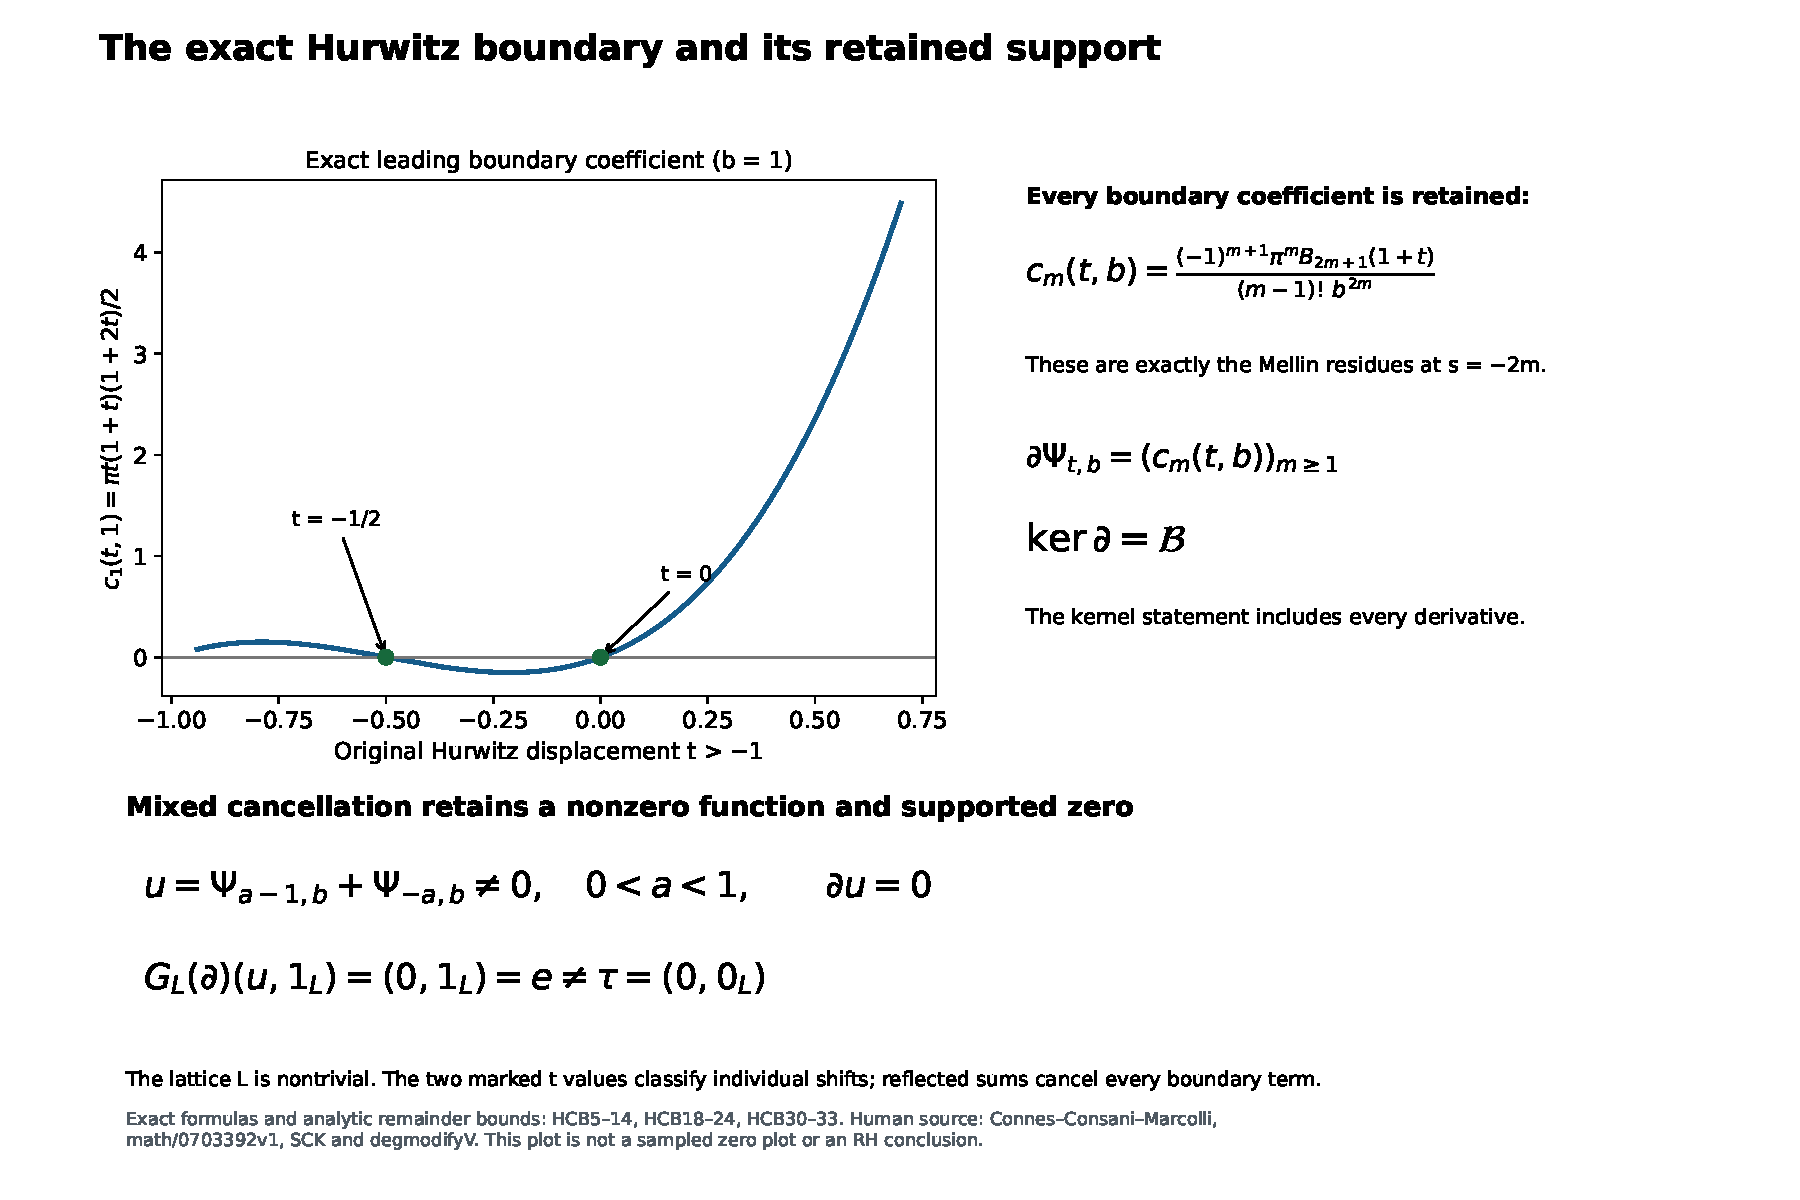
\includegraphics[width=\textwidth]{HURWITZ_WEIL_BOUNDARY.pdf}
\caption{The complete boundary is a sequence, not only its first
coordinate. The plotted first coefficient is exact at $b=1$.
Reflected mixtures cancel every coefficient while retaining
their nonzero function and supported zero.}\end{figure}
\begin{figure}[p]\centering
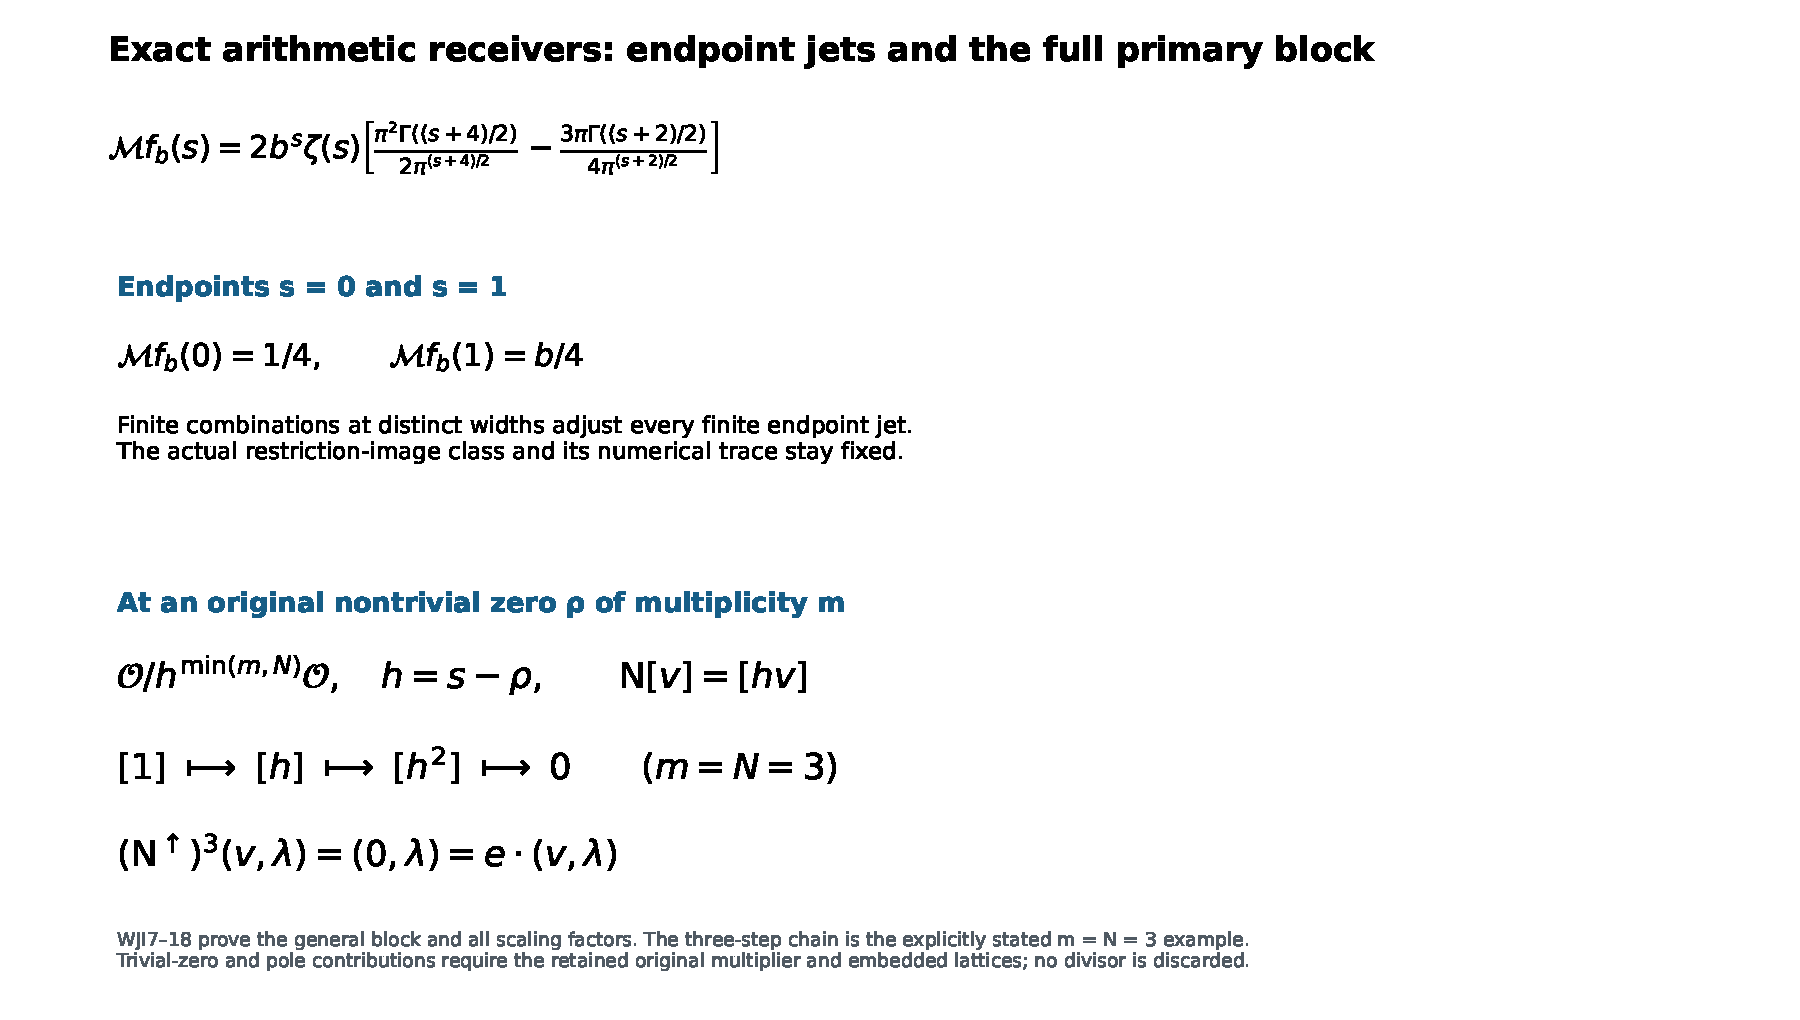
\includegraphics[width=\textwidth]{WEIL_JETS_AND_SUPPORT.pdf}
\caption{Actual restriction-image functions adjust endpoint jets
without changing the spectral class. At a nontrivial zero the full
primary block survives, including its nilpotent and its supported-zero
power. The displayed three-step example has $m=N=3$.}\end{figure}
\clearpage

% Complete programme source: ORIGINAL_ZETA_THETA_CORRECTION.tex
% ZTC: original zeta, original shifted arithmetic family, retained theta data.
\section{Original zeta and the retained theta comparison}
\label{sec:original-zeta-theta-correction}

\paragraph{Correction and provenance.}
The statement that the Rodgers--Tao heat kernel was the programme's
original construction over the entire absolute base was not established.
THS1--31 begin with that classical analytic kernel and construct a
support-preserving coefficient lift. HTB1--35 establish its exact
comparison with the shifted Hurwitz family. Neither construction is a
derivation of the scalar kernel from the entire arithmetic geometry.
The distinction is measurable: THS22 already proves that all supported
zero times act identically on the actual theta orbit. The ambient
coefficient injection does not make that orbit injective.

The original arithmetic functions in this calculation remain
\begin{equation}\tag{ZTC1}
 \zeta(s)=\sum_{n=1}^{\infty}n^{-s},\qquad
 F_t(s)=\sum_{n=0}^{\infty}(n+1+t)^{-s},
 \qquad \operatorname{Re}s>1,\quad t>-1.
\end{equation}
Their continuations, endpoints, and exact shift generator are proved in
HTB2--5, with the programme source identified there by version, hash,
and original theorem labels. In particular $F_0=\zeta$,
$F_1=\zeta-1$, and $\partial_tF_t(s)=-sF_t(s+1)$.
The latter family comes from the supplied April 2026 shifted-Hurwitz
programme draft, not from a proposed identification of two time variables.
Brad Rodgers and Terence Tao's
\href{https://arxiv.org/abs/1801.05914v5}{original author source},
equations \texttt{phidef}, \texttt{htdef}, \texttt{hoz}, and
\texttt{sas}, supplies the auxiliary heat kernel used in THS and HTB.
These are cited inputs, not new discoveries. The following comparisons
are derived explicitly. Their complete HTB, THS, and CFD proofs accompany
this chapter.

\subsection{A direct theta sum for the original arithmetic family}

For real $t>-1$ and $x>0$, retain the actual shifted frequencies and put
\begin{equation}\tag{ZTC2}
 K_t(x)=\sum_{n=0}^{\infty}
               e^{-\pi(n+1+t)^2x}.
\end{equation}
This is a scalar analytic representation of the stated arithmetic
family. No assertion that it determines the full support lattice is
part of this definition. For fixed $a=1+t>0$, monotonicity of the
summand as a function of $n$ gives
\begin{equation}\tag{ZTC3}
 K_t(x)\le e^{-\pi a^2x}
              +\int_0^\infty e^{-\pi(a+y)^2x}\,dy
 \le 1+\frac1{2\sqrt x}.
\end{equation}
For $x\ge1$ the same bound after retaining the first exponential
gives $K_t(x)\le C_a e^{-\pi a^2x}$, since
$(a+n)^2-a^2\ge n^2$ and
$C_a=\sum_{n\ge0}e^{-\pi((a+n)^2-a^2)}<\infty$.
Consequently the following integral converges absolutely for
$\operatorname{Re}s>1$:
\begin{equation}\tag{ZTC4}
 \int_0^\infty x^{s/2-1}K_t(x)\,dx
   =\pi^{-s/2}\Gamma(s/2)F_t(s),\qquad
 F_t(s)=\frac{\pi^{s/2}}{\Gamma(s/2)}
                \int_0^\infty x^{s/2-1}K_t(x)\,dx.
\end{equation}
Indeed, with $\sigma=\operatorname{Re}s>1$, the sum of the
absolute termwise integrals equals
$\pi^{-\sigma/2}\Gamma(\sigma/2)\sum_{n\ge0}(n+a)^{-\sigma}$.
Fubini therefore applies. Substitution $y=\pi(n+a)^2x$ in each
term proves the displayed identity with its full Gamma and pi factors.
Continuation outside that domain means the meromorphic continuation
proved in HTB4, not an assertion that the unsubtracted integral converges
there.

There is also an exact inverse recovering the kernel, not only the
arithmetic function. For every real $c>1$,
\begin{equation}\tag{ZTC4a}
 K_t(x)=\frac1{4\pi i}\int_{c-i\infty}^{c+i\infty}
       \pi^{-s/2}\Gamma(s/2)F_t(s)x^{-s/2}\,ds.
\end{equation}
Here the integral is absolutely convergent. To prove the inversion
with its constant, set $\sigma=c/2>0$ and
$g(v)=\exp(\sigma v-e^v)$. This function and all its derivatives
are integrable on $\mathbb R$: at $-\infty$ they are bounded
by a constant times $e^{\sigma v}$, and at $+\infty$ by a
polynomial in $e^v$ times $g(v)$. The substitution $u=e^v$
identifies its Fourier transform with $\Gamma(\sigma-i y)$.
Repeated integration by parts therefore bounds that Gamma factor
by $C_N(1+|y|)^{-N}$ for every fixed $N$.
Fourier inversion gives
$e^{-u}=(2\pi i)^{-1}\int_{\sigma-i\infty}^{\sigma+i\infty}
\Gamma(w)u^{-w}\,dw$. One may verify this inversion directly
by first multiplying the Fourier integrand by $e^{-\epsilon y^2}$:
the resulting expression is the convolution of $g$ with the
Gaussian approximate identity, which converges to $g$; the stated
integrable transform bound permits dominated convergence as
$\epsilon\downarrow0$. Apply the identity to
$u=\pi(n+1+t)^2x$, then put $s=2w$. The resulting factor is
$1/(4\pi i)$. Finally sum in $n$. Interchange is justified by
$\sum(n+1+t)^{-c}<\infty$ and the integrable Gamma bound.
This proves ZTC4a. ZTC4 and ZTC4a are mutual recovery formulas
for the specified original arithmetic family and its scalar
theta sums; they do not recover a support lattice from a scalar
function.

Differentiation in $t$ is locally uniform for $t$ in compact subsets
of $(-1,\infty)$ and $x$ in compact subsets of $(0,\infty)$, by
Gaussian majorants for a polynomial times $e^{-c n^2}$.
It gives the exact formula
\begin{equation}\tag{ZTC5}
 \partial_tK_t(x)=-2\pi x\sum_{n=0}^{\infty}
              (n+1+t)e^{-\pi(n+1+t)^2x}.
\end{equation}
For $\operatorname{Re}s>0$, integration of its absolute value is
bounded by a constant times $\sum(n+a)^{-\sigma-1}$, locally
uniformly in $t$. More precisely its Mellin transform is
\begin{equation}\tag{ZTC6}
 \int_0^\infty x^{s/2-1}\partial_tK_t(x)\,dx
 =-2\pi^{-s/2}\Gamma(s/2+1)F_t(s+1)
 =-s\pi^{-s/2}\Gamma(s/2)F_t(s+1).
\end{equation}
Thus the original arithmetic shift generator is represented directly,
without substituting the heat generator for it. The stated equality
extends meromorphically by HTB4--5.

The separated sheet and its entire missing summand are visible before
any transform:
\begin{equation}\tag{ZTC7}
 K_1(x)=K_0(x)-e^{-\pi x},\qquad
 D_t(s)=\zeta(s)-F_t(s),\qquad D_1(s)=1,
\end{equation}
\begin{equation}\tag{ZTC8}
 \pi^{-s/2}\Gamma(s/2)D_t(s)
   =\int_0^\infty x^{s/2-1}\bigl(K_0(x)-K_t(x)\bigr)\,dx
       \quad(\operatorname{Re}s>1).
\end{equation}
ZTC7 follows by deleting the $n=1$ summand of $K_0$; ZTC8 follows
by subtracting two absolutely convergent integrals. At $t=1$ the
integral is exactly $\pi^{-s/2}\Gamma(s/2)$, so its inverse returns
the actual constant $1$, including its amplitude and support when lifted.

\subsection{Original zeta with both Mellin endpoints retained}

At $t=0$, HTB6 proves
\begin{equation}\tag{ZTC9}
 K_0(x)=x^{-1/2}K_0(1/x)+\tfrac12x^{-1/2}-\tfrac12.
\end{equation}
Split ZTC4 at $x=1$, apply this identity only to the integral over
$(0,1)$, and substitute $y=1/x$ there. Initially
$\operatorname{Re}s>1$, and direct integration gives
\begin{equation}\tag{ZTC10}
 \zeta(s)=\frac{\pi^{s/2}}{\Gamma(s/2)}
 \left\{
 \frac1{s-1}-\frac1s
 +\int_1^\infty K_0(x)
             \left(x^{s/2-1}+x^{-(s+1)/2}\right)\,dx
 \right\}.
\end{equation}
The two separate rational terms are the transforms of the two separate
terms $x^{-1/2}/2$ and $-1/2$. The integral on $[1,\infty)$ is
entire in $s$, since exponential decay bounds every logarithmic
derivative on compact subsets of the $s$-plane. This proves the
meromorphic continuation of the identity and keeps both endpoint
contributions. Neither has been declared zero or absorbed into an
unrecorded constant.

For the original cosine heat kernel, retain
\begin{equation}\tag{ZTC11}
\begin{gathered}
 A(s)=\frac{s(s-1)}2\pi^{-s/2}\Gamma(s/2),\qquad
 s(z)=\frac12+\frac{iz}{2},\qquad z(s)=-2i(s-1/2),\\
 H_0(z)=\frac{s(z)(s(z)-1)}{16}
           \pi^{-s(z)/2}\Gamma(s(z)/2)\zeta(s(z)),\\
 \zeta(s)=\frac{16\pi^{s/2}}
                  {s(s-1)\Gamma(s/2)}H_0(z(s)).
\end{gathered}
\end{equation}
The proof is HTB6--10: the exact Mellin substitution and two
integrations by parts yield the displayed multiplier, with all
endpoint limits justified in the original convergence half-plane.
The last equality is an identity of meromorphic functions. It is
not a licence to replace the original zeta calculation by an entire
function calculation while dropping its multiplier.

\subsection{The boundary is part of the receiving object}

Let $\mathcal M_s$ and $\mathcal M_z$ be the complex vector spaces
of meromorphic functions on the respective complex planes. Retain
the linear isomorphism, already proved in HTB11,
\begin{equation}\tag{ZTC12}
 Uf(z)=\frac{A(s(z))}{8}f(s(z)),\qquad
 U^{-1}G(s)=\frac{8G(z(s))}{A(s)}.
\end{equation}
Define the joint map on the entire two-component space by
\begin{equation}\tag{ZTC13}
 \mathcal V:\mathcal M_s\oplus\mathcal M_s
          \longrightarrow\mathcal M_z\oplus\mathcal M_z,
 \qquad (F,D)\longmapsto\bigl(U(F+D),UD\bigr).
\end{equation}
It has the exact inverse
\begin{equation}\tag{ZTC14}
 \mathcal V^{-1}(H,J)
    =\left(\frac{8(H-J)\circ z}{A},\frac{8J\circ z}{A}\right).
\end{equation}
Substitution proves both compositions equal the identity; all entries
are meromorphic functions, so no undefined product of separate
singular point values is involved. On the actual arithmetic family,
\begin{equation}\tag{ZTC15}
\begin{gathered}
 J_t=UD_t,\qquad
 \mathcal V(F_t,D_t)=(H_0,J_t),\\
 F_t(s)=\frac{16\pi^{s/2}}
              {s(s-1)\Gamma(s/2)}
              \bigl(H_0(z(s))-J_t(z(s))\bigr),\\
 J_1(z)=\frac{A(s(z))}{8},\qquad
 J_t(i)=-\frac t8.
\end{gathered}
\end{equation}
For the last equality use HTB5:
$D_t(0)=\zeta(0)-F_t(0)=t$, $A(0)=-1$, and $z(0)=i$.
In particular the retained pair determines the real parameter $t$
by $t=-8J_t(i)$. All $t$ give the same first component $H_0$.
Discarding $J_t$ therefore identifies different actual arithmetic
inputs. This is an explicit failure of injectivity on the actual
programme family, not merely an example in an unrelated vector space.
On the unrestricted space the summation map $(G,J)\mapsto G+J$
has exactly the kernel $\{(B,-B):B\in\mathcal M_z\}$.

For the complete support carrier, use the common label on the
direct sum:
\begin{equation}\tag{ZTC16}
 G_L(\mathcal M_s\oplus\mathcal M_s)
   \xrightarrow{\mathcal V^\uparrow}
 G_L(\mathcal M_z\oplus\mathcal M_z),\qquad
 ((F,D),\lambda)\longmapsto(\mathcal V(F,D),\lambda).
\end{equation}
Here $G_L(V)=\{(0,\lambda):\lambda\in L\}\cup(V\times\{1_L\})$
with its original joins and meets. Additivity, compatibility with
the $G_L(\mathbb C)$ action, carrier membership, and the inverse
follow componentwise from linearity and ZTC14, as explicitly proved
in CFD11--12. This is a bijection for every bounded distributive $L$.
It does not silently replace the common label by independent labels
on two product factors. In particular $e=(0,1_L)$ and
$\tau=(0,0_L)$ remain distinct when $L$ is nontrivial.

\paragraph{The exact multiplication comparison.}
The preceding maps were declared as linear and semimodule maps.
Their injectivity does not identify the original multiplication with
ordinary multiplication of their images. This can be checked exactly,
without discarding the completion multiplier. Set
\begin{equation}\tag{ZTC16a}
 B(z)=\frac{A(s(z))}{8}
 =\frac{s(z)(s(z)-1)}{16}
       \pi^{-s(z)/2}\Gamma(s(z)/2).
\end{equation}
For meromorphic $f,g$ on the $s$-plane the two products are
\begin{equation}\tag{ZTC16b}
\begin{gathered}
 U(fg)(z)=B(z)f(s(z))g(s(z)),\\
 (Uf)(z)(Ug)(z)=B(z)^2f(s(z))g(s(z)).
\end{gathered}
\end{equation}
In particular $U1=B$, not the ordinary constant unit. The factor
$B$ is nonconstant: it has a zero at $z(1)=-i$ and poles at
$z(-2m)$, $m\ge1$. Thus ordinary multiplication is not preserved.
The exact transported product and its unit are
\begin{equation}\tag{ZTC16c}
 G\odot H=\frac{8G(z)H(z)}{A(s(z))},\qquad
 1_{\odot}(z)=\frac{A(s(z))}{8}.
\end{equation}
This formula is an identity of meromorphic functions, including
their germs at the zeros and poles of the multiplier. It is not
pointwise division of undefined singular values. Substitution
gives $(Uf)\odot(Ug)=U(fg)$. Directly,
$(G\odot H)\odot K=GHK/B^2=G\odot(H\odot K)$,
$B\odot G=G$, and distributivity follows from distributivity of
meromorphic multiplication. Together with ZTC12 this proves a
unital algebra isomorphism with the stated product.

For each local holomorphic ring $\mathcal O_{s_0}$ the affine
coordinate map identifies it with $\mathcal O_{z(s_0)}$.
Its exact image under $U$ is the embedded fractional lattice
$B\mathcal O_{z(s_0)}$. This lattice is closed under $\odot$,
since $(Bu)\odot(Bv)=Buv$, and has unit $B$.
Keeping instead the unmodified target $\mathcal O_{z(s_0)}$
can fail closure: at $s_0=1$, $B$ has a simple zero, so
$1\odot1=1/B$ is not holomorphic. This image-lattice statement
differs from the preimage lattice $A^{-1}\mathcal O$ in ZTC17:
the former transports an original holomorphic ring, whereas the
latter specifies which original meromorphic sections have a
holomorphic completed image.

The full support carrier admits the same exact comparison. Retain
its original addition, and define the target product by
\begin{equation}\tag{ZTC16d}
 (G,\lambda)\odot_L(H,\mu)
   =\left(\frac{8GH}{A\circ s},\lambda\wedge\mu\right),
 \qquad 1_{\odot_L}=(B,1_L).
\end{equation}
If the amplitude of a product is nonzero, both input amplitudes
are nonzero, hence both labels are $1_L$; this proves carrier
closure. If either amplitude is zero its output amplitude is
zero and the displayed meet retains its original label.
Associativity and distributivity follow from ZTC16c and the
meet/join laws of the bounded distributive lattice. The map
$(f,\lambda)\mapsto(Uf,\lambda)$ and its inverse therefore
give a unital semiring isomorphism from the original coefficient
semiring to this specified target, preserving $e$ and $\tau$.
An ideal $P$ is sent to its literal image $U^{\uparrow}(P)$;
closure under addition and multiplication follows by applying the
isomorphism. Its inverse proves the converse. Moreover a product
belongs to that image precisely when the corresponding original
product belongs to $P$, proving that prime ideals correspond.
This proves the exact spectrum comparison for these specified
coefficient semirings. It is not a derivation of the entire
arithmetic base from the scalar function $H_0$.

For ZTC13--16, no multiplication on pairs was specified: the
proved assertion there remains a common-label semimodule
isomorphism. Neither ordinary multiplication nor a Weil pairing
is silently inferred from that assertion.

\subsection{Local zeros, poles, and the original trace}

The earlier conversational assertion that the singular module map
had not been established was also too broad: HTB13 already proves
$A^{-1}\mathcal O\xrightarrow{U}\mathcal O$ with the affine
coordinate change. CFD1--10 now make the comparison with the
\emph{original} regular lattice and every finite jet explicit.
At a finite point let $h=s-s_0$ and $A=h^k a(h)$, $a(0)\ne0$.
Retain $I=A^{-1}\mathcal O=h^{-k}\mathcal O$ as an embedded
submodule of the meromorphic germs, and $J=I\cap\mathcal O$.
For nonzero $f\in I$ the original order is
\begin{equation}\tag{ZTC17}
 \operatorname{ord}_{s_0}f
 =\dim_{\mathbb C}(I/\mathcal O f)
  -\dim_{\mathbb C}(I/J)
  +\dim_{\mathbb C}(\mathcal O/J).
\end{equation}
This is proved by the power-of-$h$ bases in CFD6--7, without
identifying the reference lattices. At a trivial zero $s_0=-2m$,
$I=h\mathcal O$, $I/\mathcal O\zeta=0$ and
$\mathcal O/I$ has dimension $1$. At $s_0=1$,
$I=h^{-1}\mathcal O$, $I/\mathcal O\zeta=0$ and
$I/\mathcal O$ has dimension $1$. Their signs in ZTC17 give,
respectively, $+1$ and $-1$. At $s_0=0$, $A(0)=-1$ is a unit.
CFD4 provides the invertible triangular matrices recovering all
Laurent coefficients with the exact factors $8$ and $i/2$.
Keeping only the zero algebra of the completed section would give
zero in both cancelled cases; keeping these comparison modules
restores the actual divisor.

The earlier conversational explanation of the fibres requires a
further correction. The map
\begin{equation}\tag{ZTC17a}
 \mathcal O/h\mathcal O\longrightarrow
 h\mathcal O/h^2\mathcal O,\qquad [u]\longmapsto[hu]
\end{equation}
is an isomorphism of $\mathcal O$-modules. It is well-defined because
$h(h\mathcal O)=h^2\mathcal O$, surjective by the definition of
$h\mathcal O$, and injective because $hu\in h^2\mathcal O$ implies
$u\in h\mathcal O$ in the local integral domain. Its inverse is
$[hu]\mapsto[u]$. Consequently the two abstract fibres alone do
not account for the loss. What must be retained is their specified
embedding and the original reference lattice: multiplication by
$A=h^{-1}a(h)$ identifies $I=h\mathcal O$ with $\mathcal O$, but
the length-one quotient $\mathcal O/I$ records the cancelled
original zero. Replacing the entire marked comparison by the
completed section's zero quotient discards precisely that datum.
Likewise multiplication by nonzero meromorphic $A$ is an
automorphism of the meromorphic sheaf as a module. It is not
a ring automorphism for ordinary multiplication, as ZTC16b proves.
It is not an automorphism
of the fixed holomorphic lattice at its zeros and poles. These
category statements do not contradict one another.

Logarithmic differentiation gives the original trace identity
\begin{equation}\tag{ZTC18}
 \frac{\zeta'(s)}{\zeta(s)}
 =-2i\frac{H_0'(z(s))}{H_0(z(s))}
 -\frac1s-\frac1{s-1}+\frac12\log\pi-\frac12\psi(s/2).
\end{equation}
It first holds away from zeros and poles and then meromorphically;
$\psi=\Gamma'/\Gamma$. For a positively oriented finite contour
$\gamma$ avoiding all zeros and poles of the functions and all
singularities of every displayed integrand, and a holomorphic test $g$
on and inside it, multiplication by $g$ and integration gives
\begin{equation}\tag{ZTC19}
\begin{split}
 \frac1{2\pi i}\int_\gamma g\,\frac{\zeta'}\zeta\,ds
 ={}&\frac1{2\pi i}\int_\gamma
           g(s)(-2i)\frac{H_0'(z(s))}{H_0(z(s))}\,ds\\
 &-\frac1{2\pi i}\int_\gamma g(s)
   \left(\frac1s+\frac1{s-1}-\frac12\log\pi
                         +\frac12\psi(s/2)\right)ds.
\end{split}
\end{equation}
At every zero or pole, write a meromorphic function as
$(s-s_0)^r$ times a holomorphic unit. Its logarithmic derivative
then has residue $r$. The residue theorem proves that ZTC19
counts the original zeros with multiplicity and the original poles
with negative multiplicity, including every trivial zero inside
the contour. No infinite-contour limit or decay assumption is
hidden here. Extending this finite identity to a particular infinite
trace requires the actual convergence estimates of that trace.

\subsection{Two different trajectories through the same original zeta}

The original-$s$ function associated with the classical heat path is
\begin{equation}\tag{ZTC20}
 f_h^{\rm heat}(s)=\frac{16\pi^{s/2}}
                         {s(s-1)\Gamma(s/2)}H_h(z(s)),
 \qquad f_0^{\rm heat}=\zeta.
\end{equation}
CFD18--21 give its full receiving operator and prove
\begin{equation}\tag{ZTC21}
 \left.\partial_hf_h^{\rm heat}(-2)\right|_{h=0}=0,
 \qquad
 \left.\partial_tF_t(-2)\right|_{t=0}=-\frac16.
\end{equation}
For completeness, the heat equation and chain rule give
$\partial_hf=(Af)''/(4A)$. At $h=0$, $A\zeta$ is holomorphic
at $-2$ whereas $1/A$ has a simple zero there, giving the first
value. HTB5 gives the second as $2\zeta(-1)=-1/6$.
The discrepancy holds on the actual initial arithmetic function.
CFD21 further proves that all the zeros at $-2m$ remain simple
along the real heat path, while its residue at $1$ varies strictly;
the actual Hurwitz path has constant residue $1$ and values
$-B_{2m+1}(1+t)/(2m+1)$ at those points.

Thus the valid original-$\zeta$ receiver consists of the original
functions, their exact transform and inverse, the retained boundary
component, the embedded local comparison modules, and all support
labels. The scalar theta orbit by itself is a smaller observable.
These proofs neither exhibit an off-line zero of the original
$\zeta$ nor rule one out. They establish precisely which input and
which deformation a subsequent estimate is estimating.

\clearpage

% Complete programme source: CC_EXACT_TRIVIAL_CORRESPONDENCE.tex
% ETC: exact constants in the original CCM degree-adjusting test family.
\section{The original trivial-correspondence family with every Haar constant}
\label{sec:cc-exact-trivial-correspondence}

\paragraph{Human source and reading scope.}
Alain Connes, Caterina Consani, and Matilde Marcolli,
\href{https://arxiv.org/abs/math/0703392}{\emph{The Weil proof and the
geometry of the adeles class space}}, original author file
\texttt{Yuri70v2.tex}, subsection \emph{Fubini's theorem and the trivial
correspondences}, especially Lemma \texttt{degmodifyV}, supply the
polynomial Gaussian used below. The original file has SHA-256
\texttt{b1f694cb934dd4fe\allowbreak{}f829287f1a55dd8d\allowbreak{}e21c67a481e55245\allowbreak{}3c2f7e8fe0ae6fb5}.
The complete subsection, source lines 2313--2424, was read, together
with the definitions \texttt{fsharpinv}, \texttt{degcorrZf}, and
\texttt{codegcorrZf}. This calculation fixes the measures and sums over
all nonzero rational numbers; it replaces the source's unspecified
constant by a proved exact value. It does not replace the original
zeta function with a completed function, and makes no RH inference.

\subsection{Original adelic test, rational restrictions, and additive moments}

Use additive Haar measure $dx$ at infinity and
$\operatorname{vol}(\mathbb Z_p)=1$ at every finite prime. On
$C_{\mathbb Q}=\widehat{\mathbb Z}^{\times}\times\mathbb R_{>0}$
use Haar measure $du\,dy/y$, with
$\operatorname{vol}(\widehat{\mathbb Z}^{\times})=1$. Retain
\begin{equation}\tag{ETC1}
 \eta(x)=\pi x^2\left(\pi x^2-\frac32\right)e^{-\pi x^2}
        =\left(\pi^2x^4-\frac{3\pi}{2}x^2\right)e^{-\pi x^2},
 \quad k\in\bigoplus_p\mathbb Z,
 \quad N(k)=\prod_pp^{k_p},\quad a>0,
\end{equation}
and the actual tensor
\begin{equation}\tag{ETC2}
 \xi_{k,a}(x)=\eta(x_\infty/a)
                  \prod_p1_{p^{k_p}\mathbb Z_p}(x_p),
 \qquad b=\frac a{N(k)}>0.
\end{equation}
The symbol $b$ records this specified ratio; it does not change either
of the original parameters or the local factors. The finite product
of nonstandard factors defines a Bruhat--Schwartz function on the
original adeles.

The Gaussian integral and its two differentiated forms are
\begin{equation}\tag{ETC3}
 \int_{\mathbb R}e^{-\pi x^2}\,dx=1,\quad
 \int_{\mathbb R}x^2e^{-\pi x^2}\,dx=\frac1{2\pi},\quad
 \int_{\mathbb R}x^4e^{-\pi x^2}\,dx=\frac3{4\pi^2}.
\end{equation}
For example, square the first integral and use polar coordinates to
obtain one; differentiating
$\int e^{-\pi t x^2}dx=t^{-1/2}$ once and twice at $t=1$
gives the other two. Polynomial Gaussian bounds justify both
differentiations. Consequently
\begin{equation}\tag{ETC4}
 \eta(0)=0,\quad \int_{\mathbb R}\eta=\frac34-\frac34=0,
 \quad \xi_{k,a}(0)=0,\quad
 \int_{\mathbb A_{\mathbb Q}}\xi_{k,a}
 =a\prod_pp^{-k_p}\left(\frac34-\frac34\right)=0.
\end{equation}
Thus the two additive zero-moment conditions hold on the original
test, with both summands and every volume retained.

Define the reduction by the original full rational sum:
\begin{equation}\tag{ETC5}
 f_{k,a}(u,y)=(\mathcal E\xi_{k,a})(u,y)
 =\sum_{q\in\mathbb Q^\times}\xi_{k,a}(qy,(qu_p)_p).
\end{equation}
Since $u_p$ is a unit, its finite characteristic factors permit exactly
$v_p(q)\ge k_p$ at every prime. This says that $q/N(k)$ is a rational
number integral at every finite prime, hence an integer: a reduced
denominator greater than one would give a negative valuation at one
of its prime divisors. Conversely every nonzero integer satisfies
these conditions. The map $n\mapsto N(k)n$ is therefore a bijection
onto the permitted rational numbers. Since $\eta$ is even,
\begin{equation}\tag{ETC6}
 f_{k,a}(u,y)=\sum_{n\in\mathbb Z\setminus\{0\}}
             \eta\left(\frac{N(k)ny}{a}\right)
 =2\sum_{n=1}^{\infty}\eta(ny/b)=:f_b(y).
\end{equation}
The factor two is from the two rational signs. This is an exact map
of the specified family; it shows explicitly that this scalar
reduction depends on $k,a$ only through $a/N(k)$. It does not recover
the individual finite-place factors from that ratio.

\subsection{Fourier calculation, Poisson identity, and convergence}

Use the real Fourier convention
$\widehat h(v)=\int h(x)e^{-2\pi ixv}dx$ and compatible conductor
$\mathbb Z_p$ characters at finite places. Let $g(x)=e^{-\pi x^2}$.
The Fourier integral has derivative $-2\pi v\widehat g(v)$:
differentiate under the integral and integrate $g'=-2\pi xg$ by
parts. Its value at zero is one by ETC3, so $\widehat g(v)=g(v)$.
Differentiating this identity gives the complete two polynomial
transforms
\begin{equation}\tag{ETC7}
 \begin{split}
 \widehat{x^2g}(v)&=\left(\frac1{2\pi}-v^2\right)g(v),\\
 \widehat{x^4g}(v)&=
       \left(v^4-\frac3\pi v^2+\frac3{4\pi^2}\right)g(v),\\
 \widehat\eta(v)&=\left[
 \pi^2\left(v^4-\frac3\pi v^2+\frac3{4\pi^2}\right)
 -\frac{3\pi}{2}\left(\frac1{2\pi}-v^2\right)\right]g(v)
 =\eta(v).
 \end{split}
\end{equation}
These differentiations and integrations by parts have vanishing
boundary terms because every derivative is a polynomial times a
Gaussian. At a finite prime, character orthogonality gives
$\widehat{1_{p^{k_p}\mathbb Z_p}}
 =p^{-k_p}1_{p^{-k_p}\mathbb Z_p}$: the transform equals the
original ball volume on its annihilator and is zero outside it.
The real dilation contributes $a$. Hence
\begin{equation}\tag{ETC8}
 \widehat\xi_{k,a}
 =a\prod_pp^{-k_p}\,\xi_{-k,1/a}
 =\frac a{N(k)}\,\xi_{-k,1/a}.
\end{equation}
Applying Fourier twice yields the original even test: the second
coefficient is $(1/a)/N(-k)=N(k)/a$, so the two displayed coefficients
multiply to one.

For the required Poisson identity no rearrangement of a divergent
integral is used. For $r>0$, periodize $\eta(r(x+n))$ over
$n\in\mathbb Z$. Every differentiated series converges uniformly
on $x\in[0,1]$ by Schwartz bounds. Its $m$th Fourier coefficient
is $r^{-1}\widehat\eta(m/r)$, by the absolutely convergent
substitution over all intervals. These coefficients decrease faster
than any power, so their Fourier series converges absolutely to the
periodization. Evaluating at zero and using ETC7 gives
\begin{equation}\tag{ETC9}
 \sum_{n\in\mathbb Z}\eta(nr)
 =\frac1r\sum_{m\in\mathbb Z}\eta(m/r),\qquad
 f_b(y)=\frac b y f_{1/b}(1/y).
\end{equation}
The zero summand is zero on both sides because $\eta(0)=0$.
The same argument with $g$ proves its Gaussian Poisson formula.

For $y\ge1$ the series in ETC6 and each of its derivatives are
bounded by a polynomial in $y$ times $e^{-\pi y^2/b^2}$.
Indeed factor this last exponential from each term; the remaining
sum is bounded by a convergent series of a polynomial in $n$ times
$e^{-\pi(n^2-1)/b^2}$. ETC9 therefore bounds $f_b$ near zero
by a constant times $y^{-5}e^{-\pi b^2/y^2}$; its differentiated
versions have the same exponential with possibly different finite
powers of $y^{-1}$. Thus this actual reduced test and all its
multiplicative derivatives decrease faster than every power at both
ends. In particular every Mellin integral below converges absolutely
for every $s$, locally uniformly with all $s$ derivatives.

\subsection{Original-zeta Mellin formula with both Gaussian summands}

With the specified class-group measure put
\begin{equation}\tag{ETC10}
 M_b(s)=\int_{\widehat{\mathbb Z}^{\times}}du
            \int_0^\infty f_b(y)y^s\frac{dy}{y}
       =\int_0^\infty f_b(y)y^{s-1}dy.
\end{equation}
The preceding bounds prove that $M_b$ is entire. Initially for
$\operatorname{Re}s>1$, absolute Fubini is valid on ETC6, since
\[
 2\sum_{n\ge1}\int_0^\infty
    |\eta(ny/b)|y^{\operatorname{Re}s-1}dy
 =2b^{\operatorname{Re}s}\sum_{n\ge1}n^{-\operatorname{Re}s}
        \int_0^\infty|\eta(x)|x^{\operatorname{Re}s-1}dx<\infty.
\]
The local integral converges already for $\operatorname{Re}s>-2$,
as $\eta(x)=O(x^2)$ at zero. Substituting $v=\pi x^2$ into
each of the two original polynomial-Gaussian terms proves
\begin{equation}\tag{ETC11}
 \begin{split}
 \int_0^\infty\eta(x)x^{s-1}dx
 &=\frac{\pi^2}{2\pi^{(s+4)/2}}
       \Gamma\left(\frac{s+4}{2}\right)
   -\frac{3\pi}{4\pi^{(s+2)/2}}
       \Gamma\left(\frac{s+2}{2}\right),\\
 M_b(s)
 &=2\left(\frac a{N(k)}\right)^s\zeta(s)
   \left[
     \frac{\pi^2}{2\pi^{(s+4)/2}}
       \Gamma\left(\frac{s+4}{2}\right)
    -\frac{3\pi}{4\pi^{(s+2)/2}}
       \Gamma\left(\frac{s+2}{2}\right)
   \right].
 \end{split}
\end{equation}
The working expression keeps the original $\zeta(s)$, both Gamma
summands, the two rational signs, and all finite and real factors.
It continues meromorphically by the original zeta continuation
ZTC10; equality with the entire integral ETC10 proves that its
singularities are removable as a whole, without asserting that its
separate summands are entire.

For a precise comparison with the source's unspecified constant,
the two-step Gamma recurrence gives the identity
\begin{equation}\tag{ETC12}
 2\left[
     \frac{\pi^2}{2\pi^{(s+4)/2}}\Gamma\left(\frac{s+4}{2}\right)
    -\frac{3\pi}{4\pi^{(s+2)/2}}\Gamma\left(\frac{s+2}{2}\right)
 \right]
 =\frac{s(s-1)}4\pi^{-s/2}\Gamma(s/2).
\end{equation}
This is an explicit equality of the retained multiplier, not a
replacement arithmetic function. For real $u$ it yields the exact
source comparison
\begin{equation}\tag{ETC13}
 M_b(iu)=-\frac{b^{iu}}4\,u(u+i)
                   \pi^{-iu/2}\Gamma(iu/2)\zeta(iu).
\end{equation}
At removable points its value is the entire continuation specified
by ETC10. The factor $-1/4$ is for the full rational sum in ETC5.
Using only the positive integers would instead give $-1/8$ and
would not be the reduction defined in ETC5.

\subsection{Both endpoint values without an illicit interchange}

Retain the complete Gaussian theta sum, including its zero term:
\begin{equation}\tag{ETC14}
 \Theta_b(y)=\sum_{n\in\mathbb Z}e^{-\pi(ny/b)^2},\quad
 f_b(y)=\frac14\bigl(y^2\Theta_b''(y)+2y\Theta_b'(y)\bigr)
       =\frac14\bigl(y^2\Theta_b'(y)\bigr)'.
\end{equation}
For each summand this follows from
$x^2g''(x)+2xg'(x)=4\eta(x)$; the differentiated sums converge
locally uniformly. Gaussian Poisson summation as proved after ETC9
gives
$\Theta_b(y)=(b/y)\Theta_{1/b}(1/y)$.
As $y\to\infty$, $\Theta_b(y)\to1$ and
$y\Theta_b'(y),y^2\Theta_b'(y)\to0$.
As $y\downarrow0$, its leading term is $b/y$, with an
exponentially small remainder and differentiated remainders.
Consequently
\begin{equation}\tag{ETC15}
 \begin{gathered}
 \lim_{y\downarrow0}y^2\Theta_b'(y)=-b,\\
 \lim_{y\downarrow0}\bigl(y\Theta_b'(y)+\Theta_b(y)\bigr)=0,\\
 M_b(1)=\frac14[y^2\Theta_b'(y)]_{0}^{\infty}
       =\frac b4=\frac{a}{4N(k)},\\
 M_b(0)=\frac14[y\Theta_b'(y)+\Theta_b(y)]_{0}^{\infty}
       =\frac14.
 \end{gathered}
\end{equation}
Integrate first on a compact interval $[\epsilon,R]$ and then
take the endpoints; ETC9--10 guarantee convergence of the integrals,
and the displayed limits justify both passages. Thus the two endpoint
values are calculated from the actual reduced test, without assuming
special zeta values and without exchanging a nonabsolutely convergent
sum and integral.

The failure of the tempting degree interchange is quantified exactly.
Each $n\ne0$ term has integral zero in $dy$, by ETC4, but
\begin{equation}\tag{ETC16}
 \sum_{n\ne0}\int_0^\infty|\eta(ny/b)|dy
 =2b\left(\int_0^\infty|\eta(x)|dx\right)
                         \sum_{n=1}^\infty\frac1n=\infty.
\end{equation}
The coefficient integral is strictly positive because $\eta$ is
continuous and not identically zero. The codegree interchange also
lacks absolute convergence: each absolute integral with $dy/y$
equals the same positive finite number
$\int_0^\infty|\eta(x)|dx/x$, so its sum diverges. This does not
conflict with the convergent whole-test endpoint values ETC15.

\subsection{Sharp, conjugation, and two independent endpoint adjustments}

Use the source's literal involution
\begin{equation}\tag{ETC17}
 f^\sharp(u,y)=y^{-1}\overline{f(u^{-1},y^{-1})}.
\end{equation}
The tests $f_b$ are real and independent of $u$. Applying ETC9 at
$1/y$, and comparing with ETC8, proves
\begin{equation}\tag{ETC18}
 f_b^\sharp(y)=b f_{1/b}(y)
     =\mathcal E\widehat\xi_{k,a}(y),\quad
 M_{f_b^\sharp}(s)=bM_{1/b}(s)=M_b(1-s).
\end{equation}
For a general complex linear combination $f$ of these tests,
the exact formula instead is
\begin{equation}\tag{ETC19}
 M_{f^\sharp}(s)=\overline{M_f(1-\overline s)},\qquad
 M_{f^\sharp}(1)=\overline{M_f(0)}.
\end{equation}
Indeed substitute $v=1/y$ in the absolutely convergent integral
of $y^{-1}\overline{f(1/y)}y^{s-1}$; its integrand becomes
$\overline{f(v)}v^{-s}$, which is the displayed conjugated
Mellin transform. The source writes codegree both as $M_f(0)$
and as the degree of $f^\sharp$. Those values agree on its real
test functions, including every individual $f_b$ here; for complex
coefficients the latter is the conjugate of the former. The formulas
below specify which convention is being adjusted.

Define the complex-linear endpoint pair as
$(d(f),c(f))=(M_f(1),M_f(0))$. For two positive widths
$b_1\ne b_2$, both in the actual original family, ETC15 gives
\begin{equation}\tag{ETC20}
 \begin{pmatrix}d(c_1f_{b_1}+c_2f_{b_2})\\
                 c(c_1f_{b_1}+c_2f_{b_2})\end{pmatrix}
 =\frac14\begin{pmatrix}b_1&b_2\\1&1\end{pmatrix}
             \begin{pmatrix}c_1\\c_2\end{pmatrix},\qquad
 \det\left(\frac14\begin{pmatrix}b_1&b_2\\1&1\end{pmatrix}\right)
 =\frac{b_1-b_2}{16}\ne0.
\end{equation}
Thus prescribed changes $(D,C)\in\mathbb C^2$ are attained by
the explicit inverse
\begin{equation}\tag{ETC21}
 c_1=\frac{4(D-b_2C)}{b_1-b_2},\qquad
 c_2=\frac{4(b_1C-D)}{b_1-b_2}.
\end{equation}
Substitution gives $b_1c_1+b_2c_2=4D$ and $c_1+c_2=4C$,
proving the inverse without a dimension argument. Both widths may
use the same arbitrary divisor $k$ by choosing $a_i=N(k)b_i$.
The actual antecedent
$c_1\xi_{k,a_1}+c_2\xi_{k,a_2}$ still has zero value and zero
additive integral by ETC4, and its reduction is the displayed sum.
For real desired changes the coefficients are real. If instead
``codegree'' literally means $d(f^\sharp)$ for complex $f$,
replace $C$ by $\overline C$ in ETC21; ETC19 then proves the
corresponding real-linear inverse. This records the conjugation
rather than erasing it.

Finally the original adelic rational action is
\begin{equation}\tag{ETC22}
 (\alpha_r\xi)(x)=\xi(r^{-1}x),\quad
 \alpha_r\xi_{k,a}=\xi_{k+d(r),|r|_\infty a},\quad
 N(k+d(r))=|r|_\infty N(k),\quad
 \mathcal E\alpha_r\xi_{k,a}=\mathcal E\xi_{k,a}.
\end{equation}
The finite balls shift by their exact valuations; evenness of $\eta$
removes the real sign and leaves the real factor $|r|_\infty$.
The equality of $N$ follows from unique factorization of a nonzero
rational number. The last equality follows either from the retained
ratio in ETC6 or by reindexing the full rational sum $q\mapsto q/r$.
Real scaling alone changes $a$ to $\lambda a$, and hence
$f_b(y)$ to $f_{\lambda b}(y)=f_b(y/\lambda)$: its Mellin transform
acquires exactly $\lambda^s$, its degree exactly $\lambda$, and its
codegree remains unchanged. These are the actual two endpoint
coordinates used in ETC20--21, with every prime and real factor
retained. The calculation concerns this image family and its exact
adjustment maps; it does not assert positivity of a Weil pairing.

There is a two-dimensional adjustment space stable under the literal
sharp involution. Choose any $b>0$ with $b\ne1$ and put $c=1/b$.
In the basis $(f_b,f_c)$ the conjugate-linear operation is exactly
\begin{equation}\tag{ETC23}
 (z_1f_b+z_2f_c)^\sharp
 =\frac{\overline{z_2}}b f_b
       +b\overline{z_1}f_c,\qquad
 \begin{pmatrix}0&1/b\\b&0\end{pmatrix}^{\!2}=I.
\end{equation}
Both coefficients come from ETC18, including its width factor.
Define in this same space the original linear combinations
\begin{equation}\tag{ETC24}
 A_d=\frac{4(f_b-f_c)}{b-c},\qquad
 A_c=\frac{4(bf_c-cf_b)}{b-c}.
\end{equation}
Direct substitution into ETC15 proves
$(d(A_d),c(A_d))=(1,0)$ and $(d(A_c),c(A_c))=(0,1)$.
The determinant in ETC20 proves that these moments uniquely determine
an element of this two-dimensional space. ETC19 and its invariance
under sharp therefore give $A_d^\sharp=A_c$ and
$A_c^\sharp=A_d$, or equivalently
\begin{equation}\tag{ETC25}
 (D A_d+C A_c)^\sharp
       =\overline C A_d+\overline D A_c.
\end{equation}
These are explicit combinations of the two original tests and their
actual rational reductions. In particular they supply every prescribed
endpoint pair while retaining the involution and the original
zero-additive-moment antecedents.

For completeness, the two Gamma contributions in ETC11 have the
following separate behavior at the two endpoint arguments. Write
$h=s-1$ and $\zeta(s)=h^{-1}+c_0+O(h)$, where $c_0$ denotes its
retained Laurent constant. Set $L_b=\log b-\tfrac12\log\pi$.
The first Gamma summand including its factors has expansion
\begin{equation}\tag{ETC26}
 \begin{split}
 b^s\pi^{-s/2}\Gamma(s/2+2)\zeta(s)
 &=\frac{3b}{4h}+\frac{3b}{4}(c_0+L_b)
                     +\frac{b}{2\sqrt\pi}\Gamma'(5/2)+O(h),\\
 -\frac32b^s\pi^{-s/2}\Gamma(s/2+1)\zeta(s)
 &=-\frac{3b}{4h}-\frac{3b}{4}(c_0+L_b)
                     -\frac{3b}{4\sqrt\pi}\Gamma'(3/2)+O(h).
 \end{split}
\end{equation}
The Gamma recurrence differentiated at $3/2$ gives
$\Gamma'(5/2)=\tfrac32\Gamma'(3/2)+\Gamma(3/2)$.
Adding the two displayed expansions therefore retains and cancels
their opposite residues and their equal Laurent and width constants,
leaving exactly $b/4$. At $s=0$ the two summands have values
$\zeta(0)$ and $-\tfrac32\zeta(0)$. Their bracket is $-1/2$;
ETC15 and ETC11 imply $\zeta(0)=-1/2$, so their separate values
are $-1/2$ and $3/4$. Their sum is the independently calculated
$1/4$. Thus neither endpoint calculation has discarded the
contribution of one original Gaussian term.

\clearpage

% Complete programme source: CC_SUPPORTED_WEIL_QUOTIENT.tex
% SWQ: independent derivation, 2026-09-23.
\section{The original adelic trace quotient with every support label retained}
\label{sec:cc-supported-weil-quotient}

\paragraph{Human sources, objects, and reading scope.}
The analytic input is Alain Connes, Caterina Consani, and Matilde
Marcolli, \href{https://arxiv.org/abs/math/0703392v1}{\emph{The Weil proof
and the geometry of the adeles class space}}, original author file
\texttt{Yuri70v2.tex}, SHA-256
\texttt{b1f694cb934dd4fe\allowbreak{}f829287f1a55dd8d\allowbreak{}e21c67a481e55245\allowbreak{}3c2f7e8fe0ae6fb5},
canonical programme source \texttt{PUBUNIT-5DE2A2D44F8B1470AC701FDA}.
The sections actually read for this derivation are source lines
610--710, 1316--1425, 1508--1551, 1680--1830, 1980--2160,
2161--2216, and 2313--2424, together with the title and author lines.
The original locators are \texttt{SCK}, \texttt{rangeTrpi},
\texttt{rangecVdef}, \texttt{varthetaH1V},
\texttt{varthetafconvol}, \texttt{vanishV},
\texttt{tracepairing}, \texttt{fsharpinv},
\texttt{TraceformulaThm}, and \texttt{TraceformulaH1}.
The paragraph following \texttt{motH1AKCK} specifies closure of
the range in the cokernel. The trace-class and explicit-formula
theorems are cited analytic inputs. The convolution ideal, its sharp
invariance with all endpoint terms, and the full-label quotient and
receiving maps are derived below. No positivity assertion or RH
conclusion is made.

\subsection{The original test algebra and its domains}

Retain the source's unscaled test algebra and operations:
\begin{equation}\tag{SWQ1}
\begin{gathered}
 C=\mathbb A_{\mathbb Q}^{\times}/\mathbb Q^{\times},\qquad
 B=\bigcap_{\beta\in\mathbb R}|\cdot|^\beta\mathcal S(C),\\
 (f*g)(x)=\int_C f(h)g(h^{-1}x)\,d^{\times}h,\qquad
 f^{\sharp}(x)=|x|^{-1}\overline{f(x^{-1})}.
\end{gathered}
\end{equation}
For $\mathbb Q$, the actual continuous multiplicative section in
the author's subsection \texttt{XKCKsect} is
\begin{equation}\tag{SWQ2}
 C=\mathbb R_{>0}\times K,\qquad K=\widehat{\mathbb Z}^{\times},
 \qquad (r,u)\longmapsto(r,(u_p)_p),
 \qquad |(r,u)|=r.
\end{equation}
Indeed one multiplies an idele by the unique rational number that
makes every finite component a unit and its real component positive.
The ambiguity would have all finite valuations zero and positive real
component, so would be the rational number $1$. Multiplication
respects these representatives. The multiplicative Haar measure is
$dr/r\,du$, where $\int_Kdu=1$. The additive adelic measure is real
Lebesgue measure times the measures of volume $1$ on each
$\mathbb Z_p$. These exact measures are retained throughout.

The topology used for closure below is the usual weighted Bruhat
test-function topology: at each fixed open subgroup $H\subset K$,
functions are $H$-invariant and have all weighted Schwartz seminorms;
one then uses the Bruhat inductive-limit topology over these finite
levels. An explicit defining family at a fixed level, with $r=e^x$, is
\begin{equation}\tag{SWQ3}
 p_{N,m,j}(f)=\sup_{x\in\mathbb R,\ u\in K}
 e^{N|x|}(1+|x|)^m
 \left|\partial_x^j f(e^x,u)\right|,
 \quad N,m,j\in\mathbb Z_{\ge0}.
\end{equation}
These seminorms retain all real weights in SWQ1: weights $e^{\beta x}$
are bounded by $e^{N|x|}$ when $N\ge|\beta|$, and conversely the two
weights $e^{Nx}$ and $e^{-Nx}$ control $e^{N|x|}$; Leibniz's formula
controls their derivatives. This is a description of the original
test domain, not a change of function or scale in its operations.

All convolution integrals in SWQ1 converge absolutely. Using
$x=y+(x-y)$ and $1+|x|\le(1+|y|)(1+|x-y|)$ gives the explicit bound
\begin{equation}\tag{SWQ4}
 p_{N,m,j}(f*g)
 \le 2p_{N+1,m,0}(f)\,p_{N,m,j}(g).
\end{equation}
The constant $2$ is $\int_{\mathbb R}e^{-|y|}dy$; the compact Haar
factor is $1$. Differentiation can pass under the integral by the
same bound on every derivative. Convolution preserves a common
finite level, and this proves the continuity needed below. Since
$C$ is abelian, substitution $h\mapsto xh^{-1}$ proves commutativity.
Fubini, justified by the corresponding three-function $L^1$ bound,
proves associativity.

In these coordinates sharp is exactly
\begin{equation}\tag{SWQ5}
 f^{\sharp}(e^x,u)=e^{-x}\overline{f(e^{-x},u^{-1})},\qquad
 p_{N,m,j}(f^{\sharp})\le
 \sum_{\ell=0}^j\binom j\ell p_{N+1,m,\ell}(f).
\end{equation}
The bound follows by differentiating $e^{-x}$ and $f(e^{-x},u^{-1})$;
the two derivative signs together have absolute value $1$.
Direct substitution gives $(f^{\sharp})^{\sharp}=f$.
Inversion preserves Haar measure on this abelian group, and the norm
is a character. Substitution in the absolutely convergent convolution
therefore gives $(f*g)^{\sharp}=g^{\sharp}*f^{\sharp}$.
In particular sharp is continuous on the stated test space.
The algebra $B$ has no convolution unit among its functions.
Indeed let $b(e^x,u)=e^{-x^2}$, which belongs to $B$ and has
trivial compact-unit character. Its real Fourier transform is
$\sqrt\pi e^{-t^2/4}$, nonzero for every real $t$. A convolution
unit $a\in B$ would consequently have
$\int_{\mathbb R\times K}a(e^x,u)e^{itx}\,dx\,du=1$ for every
$t$. Integration by parts in $x$, justified by SWQ3, makes this
integral tend to zero as $|t|\to\infty$, a contradiction.
No unit distribution is inserted in this chapter.

\subsection{The adelic source, with both Poisson endpoints}

Use the canonical additive character trivial on $\mathbb Q$, with
real component $e^{-2\pi ixy}$ and finite conductor $\mathbb Z_p$,
and its self-dual measures specified after SWQ2. Write
\begin{equation}\tag{SWQ6}
\begin{gathered}
 \widehat\xi(y)=\int_{\mathbb A}\xi(x)\alpha(xy)\,dx,
 \qquad \varepsilon_0(\xi)=\xi(0),\qquad
 \varepsilon_1(\xi)=\int_{\mathbb A}\xi(x)\,dx,\\
 \mathcal S(\mathbb A)_0=\ker\varepsilon_0\cap\ker\varepsilon_1,
 \qquad (E\xi)(g)=\sum_{q\in\mathbb Q^{\times}}\xi(qg),
 \qquad V=E\mathcal S(\mathbb A)_0.
\end{gathered}
\end{equation}
For the reference characters $e_v$ in SWQ28, choose exactly
these local components of $\alpha$. This fixes more than their
conductors: it specifies the characters themselves, so that
the differential idele there is $a_v=1$ at every place.
The sum is invariant under the rational choice of representative.
For fixed $g$, finite-place compact support puts its contributing
rational $q$ in $D^{-1}\mathbb Z$ for one positive integer $D$.
Real Schwartz decay then makes the sum absolutely convergent,
locally uniformly with every real derivative. Unit dilation at
finite places preserves the required common denominator and bounds.

For completeness the full Poisson formula used here is
\begin{equation}\tag{SWQ7}
 \sum_{q\in\mathbb Q}\xi(qg)
   =|g|^{-1}\sum_{q\in\mathbb Q}\widehat\xi(qg^{-1}).
\end{equation}
It follows directly for the original Bruhat space. A finite-place
test function is a finite linear combination of characteristic
functions of cosets $a+N\widehat{\mathbb Z}$, with rational $a$ and
positive integer $N$, after a common denominator is chosen. The
rational elements in such a coset are $a+N\mathbb Z$. Real
periodization of a Schwartz function gives
\[
 \sum_{n\in\mathbb Z}\phi(a+Nn)
  =\frac1N\sum_{m\in\mathbb Z}
       e^{2\pi i ma/N}\widehat\phi(m/N).
\]
To verify this last identity, periodize over $N\mathbb Z$, integrate
over one period to compute every Fourier coefficient, and evaluate
the resulting absolutely convergent Fourier series at $a$.
The finite Fourier transform of the characteristic coset is
$N^{-1}\alpha_f(ay)1_{N^{-1}\widehat{\mathbb Z}}(y)$.
At rational $y=m/N$, its character is $e^{2\pi i am/N}$ because
the global character is trivial on rational numbers. These exact
factors prove adelic Poisson by linearity. Finally replacing the
test function by $x\mapsto\xi(gx)$ multiplies its Fourier transform
by $|g|^{-1}$ and evaluates it at $g^{-1}y$, proving SWQ7.
The same real Fourier inversion and finite character orthogonality
give $\widehat{\widehat\xi}(x)=\xi(-x)$.

Separating the actual $q=0$ terms in SWQ7, with neither endpoint
discarded, gives
\begin{equation}\tag{SWQ8}
 E\xi(g)=|g|^{-1}E\widehat\xi(g^{-1})
             +|g|^{-1}\varepsilon_1(\xi)-\varepsilon_0(\xi).
\end{equation}
For $|g|\ge1$, the earlier common-denominator estimate gives
$E\xi(g)=O_M(|g|^{-M})$ for every $M$, uniformly in the compact
unit coordinate and with every logarithmic real derivative.
For $\xi\in\mathcal S(\mathbb A)_0$, both displayed endpoints
vanish by definition, and the right side applies the same large-norm
estimate to $\widehat\xi$ at $g^{-1}$. Indeed
$\widehat\xi(0)=\varepsilon_1(\xi)=0$ and
$\int\widehat\xi=\xi(0)=0$ by Fourier inversion.
The factor $|g|^{-1}$ stays present. Since $M$ is arbitrary, it
proves all the small-norm bounds in SWQ3 as well. Thus $V\subset B$
on the source's actual domain.

Apply SWQ8 to $\widehat{\overline\xi}$, or equivalently apply
SWQ7 to $\overline\xi$ and invert $g$. The exact result is
\begin{equation}\tag{SWQ9}
 (E\xi)^{\sharp}(g)
 =E\widehat{\overline\xi}(g)
      -|g|^{-1}\overline{\varepsilon_0(\xi)}
      +\overline{\varepsilon_1(\xi)}.
\end{equation}
This identity retains the conjugations, the factor $|g|^{-1}$,
and both endpoints. Put $J\xi=\widehat{\overline\xi}$. Its
endpoints are
\begin{equation}\tag{SWQ10}
 \varepsilon_0(J\xi)=\overline{\varepsilon_1(\xi)},\qquad
 \varepsilon_1(J\xi)=\overline{\varepsilon_0(\xi)}.
\end{equation}
Consequently $J$ preserves the actual space $\mathcal S(\mathbb A)_0$
and SWQ9 gives $V^{\sharp}\subset V$; applying sharp twice gives
equality. This derives sharp invariance from additive Fourier--Poisson,
rather than assuming that the original quotient was an involutive
quotient.

\subsection{The actual convolution ideal and its closure}

For $f\in B$, $\xi\in\mathcal S(\mathbb A)_0$, use the actual
multiplicative section SWQ2 to define
\begin{equation}\tag{SWQ11}
 \eta(x)=\int_C f(h)\xi(h^{-1}x)\,d^{\times}h.
\end{equation}
This integral belongs to the original Bruhat--Schwartz space.
Indeed the orbit of the finite-place component of $\xi$ under
the compact group $K$ lies in a finite-dimensional space of test
functions: its compact support stays in one finite product of
bounded balls, and its common local-constancy subgroups are unchanged
by units. The finite quotient of this compact support by these
subgroups has finitely many points. For the real component, every
Schwartz seminorm has the explicit bound
\begin{equation}\tag{SWQ12}
 \sup_{x_\infty,x_f}
 |x_\infty^N\partial_{x_\infty}^j\eta(x)|
 \le C_{\xi,N,j}\int_C |f(h)|\,|h|^{N-j}\,d^{\times}h<\infty.
\end{equation}
The last integral is finite by SWQ3. Differentiation and integration
are justified by the same bound, while the fixed finite-place
test space makes the resulting function a Bruhat test function.

The two endpoints of this integral are exactly
\begin{equation}\tag{SWQ13}
 \eta(0)=\varepsilon_0(\xi)\int_C f(h)\,d^{\times}h,\qquad
 \int_{\mathbb A}\eta(x)\,dx
 =\varepsilon_1(\xi)\int_C |h|f(h)\,d^{\times}h.
\end{equation}
For the second equation the absolute double integral is bounded by
$\|\xi\|_{L^1(\mathbb A)}\int_C|h||f(h)|d^{\times}h$, which is
finite. The change of variables $x=hy$ therefore gives its exact
adelic factor $|h|$, and Fubini is valid for this equation.
Thus $\eta\in\mathcal S(\mathbb A)_0$.

There is also a justified interchange with the arithmetic sum in
the convolution calculation. For fixed $g$, real Schwartz decay and
the fixed rational denominator give, uniformly in the unit part of
$h$, the estimate
\[
 \sum_{q\ne0}|\xi(qh^{-1}g)|\le C_{\xi,g}(1+|h|).
\]
For example, dominate the real values on the grid $D^{-1}\mathbb Z$
by $C(1+|n||g|/(D|h|))^{-2}$, and bound the resulting series by
its first term plus its integral. Multiplying by $|f(h)|$ is
integrable by SWQ3. Hence
\begin{equation}\tag{SWQ14}
 f*E\xi=E\eta\in V.
\end{equation}
Commutativity gives the ideal property in both orders. This proves
the actual ideal assertion needed for the quotient, including the
source-domain check in Lemma \texttt{varthetaH1V}.

Let
\begin{equation}\tag{SWQ15}
 W=\overline V\subset B,\qquad Q=B/W,
\end{equation}
where closure is in the topology stated before SWQ3. Continuity of
convolution by each fixed test function, established in SWQ4,
makes $W$ a convolution ideal. Continuity and involutivity of
sharp in SWQ5, together with SWQ9--10, give $W^{\sharp}=W$.
Thus
$[f]*[g]=[f*g]$ and $[f]^{\sharp}=[f^{\sharp}]$
are well-defined on $Q$. Notice that SWQ13 is not an exchange of
$\sum_{q\ne0}$ with the degree integral of $E\xi$. It does not
assert $\int_C|g|E\xi(g)d^{\times}g=0$. The author's
\texttt{fubini1}--\texttt{nothappen} calculation concerns precisely
that different, generally invalid exchange.

\subsection{The full-label quotient and the different Bourne quotient}

Let $L$ be any bounded distributive lattice. All constructions below
hold without finiteness; to require $e\ne\tau$ take $L$ nontrivial.
Define the original constrained carrier and operations
\begin{equation}\tag{SWQ16}
\begin{gathered}
 G_L(B)=\{(0,\lambda):\lambda\in L\}\cup(B\times\{1_L\}),\\
 (f,\lambda)+(g,\mu)=(f+g,\lambda\vee\mu),\qquad
 (f,\lambda)*(g,\mu)=(f*g,\lambda\wedge\mu),\\
 (f,\lambda)^{\sharp}=(f^{\sharp},\lambda),\qquad
 \tau=(0,0_L),\quad e=(0,1_L).
\end{gathered}
\end{equation}
This is a commutative nonunital convolution semiring with sharp.
Carrier closure follows because any nonzero output amplitude requires
all relevant nonzero input amplitudes to have top label. For the
product this uses that convolution with a zero function is zero;
it does not assume that $B$ has no zero divisors. Associativity and
distributivity combine those of convolution with the lattice laws.
Sharp is an involution preserving labels and reversing convolution.
The complex scalar action has the separate semimodule formula
$(c,\alpha)(f,\lambda)=(cf,\alpha\wedge\lambda)$ for
$(c,\alpha)\in G_L(\mathbb C)$.

The exact same-label quotient is
\begin{equation}\tag{SWQ17}
 (f,\lambda)\sim_W(g,\mu)\quad\Longleftrightarrow\quad
 \lambda=\mu\ \hbox{and}\ f-g\in W,
 \qquad G_L(B)/\!\sim_W\ \simeq G_L(Q).
\end{equation}
To prove this, use the map
$\pi_L(f,\lambda)=([f],\lambda)$. It respects addition,
convolution, sharp, and the scalar action by the ideal and
involution properties just proved. It is onto: a nonzero quotient
amplitude has top label and lifts to a representative with top label;
a zero amplitude with any label lifts to $(0,\lambda)$.
Its fibres are exactly the displayed relation. Alternatively, adding
a third element preserves equality of labels and preserves the
amplitude difference modulo $W$; multiplication sends that difference
to an element of $W$; sharp sends it into $W$ as well. These direct
checks prove the required congruence and the quotient assertion.

In particular every $(0,\lambda)$ survives, and $e$ and $\tau$
remain distinct for nontrivial $L$. A nonzero $w\in W$ with top
label maps to $e$, which differs from $\tau$ when $L$ is nontrivial.
For nontrivial $L$, the inverse image of the absorbing
additive zero $\tau$ under $\pi_L$ is only $\{\tau\}$, even though
$\pi_L$ can identify different top-labelled amplitudes. Thus the
preimage of a single zero does not specify this semiring congruence.
For the one-element lattice instead $G_L(B)=B$, and that inverse
image is the ordinary amplitude kernel $W$.

The ordinary Bourne congruence by the ideal $I=G_L(W)$ is different:
\begin{equation}\tag{SWQ18}
 x\equiv_I y\quad\Longleftrightarrow\quad
 \exists a,b\in I:\ x+a=y+b,
 \qquad
 (f,\lambda)\equiv_I(g,\mu)\Longleftrightarrow f-g\in W.
\end{equation}
The forward implication follows from the amplitude equation.
Conversely, if $f-g\in W$, choose
$a=(g-f,1_L)$ and $b=(0,1_L)$. Both belong to $I$; the two
amplitudes become $g$ and both labels become $1_L$, proving equality.
Consequently
\begin{equation}\tag{SWQ19}
 G_L(B)/\!\equiv_I\ \simeq Q,
 \qquad
 G_L(B)/\!\sim_W\ \longrightarrow Q,
 \quad([f],\lambda)\longmapsto[f].
\end{equation}
The Bourne quotient collapses the entire labelled-zero fibre, so it
identifies $e$ and $\tau$. More exactly it is the same-label quotient
followed by the congruence generated by $e=\tau$: multiplication
of this equality by $(0,\lambda)$ makes $(0,\lambda)=\tau$ for
every $\lambda$. After these identifications the carrier and
operations are exactly those of $Q$. No Boolean character or
selected support point has been used.

\subsection{Every numerical additive trace and the full-labelled receiver}

Let $A$ be any abelian group. Every additive map
$t:G_L(B)\to A$ kills every labelled zero: its idempotence gives
$t(0,\lambda)+t(0,\lambda)=t(0,\lambda)$, hence $t(0,\lambda)=0$.
Define $\ell(f)=t(f,1_L)$. Then $\ell$ is additive on $B$, since
addition of two top-labelled elements stays top-labelled and
$\ell(0)=t(e)=0$. Every nonzero amplitude already has top label,
so
\begin{equation}\tag{SWQ20}
 t(f,\lambda)=\ell(f),\qquad
 \operatorname{Hom}_{+}(G_L(B),A)
       \simeq\operatorname{Hom}_{+}(B,A).
\end{equation}
Conversely composition of any additive $\ell$ with amplitude
projection is additive, proving both directions. This includes all
numerical additive traces into $\mathbb C$, not only continuous or
complex-linear ones. Cyclicity adds no restriction here because
convolution is commutative. Such a map descends through SWQ17
exactly when $\ell(W)=0$: necessity follows by comparing $(w,1_L)$
with $e$, and sufficiency follows from the displayed difference
condition. The same classification on $G_L(Q)$ is
$\operatorname{Hom}_{+}(G_L(Q),A)=\operatorname{Hom}_{+}(Q,A)$.
Thus numerical additivity itself removes zero-label distinctions;
it is not a proof that those distinctions were absent from the
source object.

Retain the original numerical cohomological trace
\begin{equation}\tag{SWQ21}
 T(f)=\operatorname{Tr}\bigl(\underline\vartheta_m(f)\mid H^1\bigr).
\end{equation}
Here $\underline\vartheta_m(f)$ is the original convolution action
on the source's quotient realization, with its prescribed closure.
Its trace-class meaning is the cited Theorem
\texttt{varthetagTrH1}, with the trace formula
\texttt{TraceformulaThm}; this chapter does not replace that
analytic theorem by a finite-dimensional trace assumption.
Its vanishing on $W$ can be checked on the actual quotient action:
for $w\in W$ and $b\in B$, $w*b\in W$, hence
$\underline\vartheta_m(w)[b]=0$. The operator is zero, so
\begin{equation}\tag{SWQ22}
 T(W)=0,\qquad \overline T:Q\to\mathbb C,\quad
 \overline T([f])=T(f).
\end{equation}
This does not require an unproved exchange of an infinite spectral
sum with a limit of representatives: the operator itself vanishes.

The original trace and Weil-pairing receivers retaining the labels are
\begin{equation}\tag{SWQ23}
\begin{gathered}
 T_L:G_L(Q)\longrightarrow G_L(\mathbb C),\qquad
 T_L([f],\lambda)=(T(f),\lambda),\\
 \mathcal W_L\bigl(([f],\lambda),([g],\mu)\bigr)
   =\bigl(T(f*g^{\sharp}),\lambda\wedge\mu\bigr).
\end{gathered}
\end{equation}
The first map is well-defined by SWQ22. It respects addition and
the declared $G_L(\mathbb C)$ scalar action; it is a trace receiver,
not a claimed multiplicative character. For the second, replace
$f$ by $f+w$ and $g$ by $g+v$, with $w,v\in W$. Its change of
amplitude is
\begin{equation}\tag{SWQ24}
 T\bigl(w*g^{\sharp}+f*v^{\sharp}+w*v^{\sharp}\bigr)=0.
\end{equation}
Every summand belongs to $W$ by SWQ15. This proves representative
independence while retaining each term of the actual change.
If one input quotient amplitude is zero, the output amplitude is
zero. Thus every nonzero output amplitude has top label and the
receiver belongs to the declared constrained carrier.

The receiver is additive in both variables and complex-linear in
the first, conjugate-linear in the second, with the exact lattice
factors. For example, if $a=(c,\alpha)$, then
\begin{equation}\tag{SWQ25}
 \mathcal W_L(ax,y)=a\mathcal W_L(x,y),\qquad
 \mathcal W_L(x,ay)=\overline a\,\mathcal W_L(x,y),
 \quad\overline a=(\overline c,\alpha).
\end{equation}
The amplitudes follow from convolution and sharp. For additivity,
the label equality is
$(\lambda\vee\lambda')\wedge\mu
=(\lambda\wedge\mu)\vee(\lambda'\wedge\mu)$, and likewise in
the second variable. These prove the assertions directly.
In particular
$\mathcal W_L((0,\lambda),([g],\mu))=(0,\lambda\wedge\mu)$.
Even a zero numerical amplitude therefore retains its exact support
in SWQ23. Projecting to $\mathbb C$ forgets that support by SWQ20.

\subsection{The complete original trace terms of this receiver}

For the trivial unit character write
$M f(s)=\int_C f(u)|u|^s d^{\times}u$. Every such integral
converges absolutely on the full complex plane by SWQ3, locally
uniformly with every derivative. Haar inversion gives
\begin{equation}\tag{SWQ26}
 M(f^{\sharp})(s)=\overline{M f(1-\overline s)},\qquad
 M(f*g^{\sharp})(s)=M f(s)\overline{M g(1-\overline s)}.
\end{equation}
For the second identity the weighted double integral is finite,
so multiplicative Fubini is valid. At the identity one has instead
the exact weighted inner-product expression
\begin{equation}\tag{SWQ27}
 (f*g^{\sharp})(1)
    =\int_C f(u)\overline{g(u)}|u|\,d^{\times}u.
\end{equation}
In particular $M(f^{\sharp})(1)=\overline{M f(0)}$.
The conjugation is necessary for complex tests; it is missing in
the author's displayed \texttt{codegcorrZf} equality if that equality
is read for unrestricted complex-valued $f$. No real-valued
restriction is imposed here.

Put $h=f*g^{\sharp}$. The source's full trace formula therefore
gives the following amplitude for SWQ23:
\begin{equation}\tag{SWQ28}
\begin{split}
 T(h)={}&M f(0)\overline{M g(1)}
       +M f(1)\overline{M g(0)}\\
 &-(\log|a|)\int_C f(u)\overline{g(u)}|u|d^{\times}u\\
 &-\sum_{v\le\infty}\int_{(\mathbb Q_v^{\times},e_v)}'
                \frac{h(u^{-1})}{|1-u|_v}\,d_v^{\times}u.
\end{split}
\end{equation}
Here $u$ denotes the idele class of its original local embedding,
$a$ is the differential idele relating the global additive character
to the specified local characters, and $d_v^{\times}u$ and the
primed distributions are exactly those of
\texttt{TraceformulaH1} and \texttt{princvalrhobeta}.
In the canonical rational character used in SWQ6 one has $a_v=1$
at every place, so the displayed differential term evaluates with
$\log|a|=\log1=0$; it has not been absorbed into another term.
The prime sum includes infinity and every finite prime.

The prime notation is essential. In the author's definition a
distribution $\varrho_{e_v}$ extends multiplicative measure across
zero with Fourier transform satisfying
$\widehat\varrho_{e_v}(1)=0$, and the local term is
\[
 \left\langle\varrho_{e_v},
   \lambda\longmapsto
       \frac{h((\lambda+1)^{-1})}{|\lambda+1|_v}\right\rangle.
\]
For compactly supported tests this is the stated original definition;
for the full space $B$, SWQ28 uses the extension on that test space
in the cited trace theorem. It is not an assertion that the ordinary
integral through $u=1$ converges. No replacement of $f$ by
$|\cdot|^{1/2}f$, and no completed zeta function, is introduced
into SWQ23--28.

\paragraph{Exact scope and analytic limits.}
The closure in SWQ15 is the declared weighted Bruhat closure, not
an unspecified Hilbert, distributional, or pointwise closure.
The quotient, ideal, and sharp statements above are proved in this
domain. The scalar trace-class realization and its regularized
explicit formula retain the analytic hypotheses of the original
source theorems. SWQ23 does not supply a new proof of those input
theorems or a positivity result. It supplies a fully specified
same-label receiving object and proves how its operations and every
trace term descend. Its numerical values are exactly the original
ones: every such value is attained on top-labelled inputs, and every
labelled input has the displayed numerical amplitude. The support
data remain in $G_L(Q)$ and in $G_L(\mathbb C)$; an additive
numerical observation necessarily forgets them by SWQ20. The Bourne
quotient performs that forgetting already in its source, whereas
SWQ17 retains $e\ne\tau$ for every nontrivial $L$.

\clearpage

% Complete programme source: CC_WEIL_JET_INTERPOLATION.tex
% WJI: exact finite jets of actual adelic trivial correspondences.
\section{Actual trivial correspondences, spectral jets, and supported nilpotence}
\label{sec:cc-weil-jet-interpolation}

\paragraph{Source and scope.}
Alain Connes, Caterina Consani and Matilde Marcolli,
\href{https://arxiv.org/abs/math/0703392v1}{\emph{The Weil proof and the
geometry of the adeles class space}}, original author file
\texttt{Yuri70v2.tex}, define the restriction image in
\texttt{rangecVdef}, the induced convolution action in
\texttt{varthetafconvol}, and prove its trace vanishing in
\texttt{vanishV}. Their \texttt{degmodifyV} uses the particular
Schwartz function below, stating its transform only up to a
constant factor. The factor is retained here. The interpolation
and support calculations are the following programme derivation,
not a claim that these proofs occur verbatim in that source.

Let $k=(k_p)_p$ have finite support in $\bigoplus_p\mathbb Z$,
let $a>0$, and retain
\begin{equation}\tag{WJI1}
 N(k)=\prod_p p^{k_p},\qquad
 \eta(x)=\pi x^2(\pi x^2-\tfrac32)e^{-\pi x^2},\qquad
 \xi_{k,a}(x)=\eta(x_\infty/a)
                     \prod_p{\bf1}_{p^{k_p}\mathbb Z_p}(x_p).
\end{equation}
The additive Haar measures have
$\operatorname{vol}(\mathbb Z_p)=1$; on
$C_{\mathbb Q}=\widehat{\mathbb Z}^{\,*}\times\mathbb R_+^*$
retain Haar mass one on $\widehat{\mathbb Z}^{\,*}$ and $dy/y$.
Here $\xi_{k,a}(0)=0$ and its additive integral is zero:
the two real Gaussian moments are
$\pi^2\cdot3/(4\pi^2)$ and $(3\pi/2)\cdot1/(2\pi)$,
and their difference is zero. The finite Haar factor is
$N(k)^{-1}$ and the real change of variable contributes $a$;
neither factor has been discarded.

For $u\in\widehat{\mathbb Z}^{\,*}$ put
\begin{equation}\tag{WJI2}
 f_b(u,y)=E\xi_{k,a}(u,y)
   =\sum_{q\in\mathbb Q^*}\xi_{k,a}(q(u,y))
   =2\sum_{n\ge1}\eta(ny/b),\qquad b=a/N(k).
\end{equation}
Indeed the finite factors require $q\in N(k)\mathbb Z$,
and $\eta$ is even. This proves the factor $2$ and the exact
relation of $b$ to every original prime valuation and real width.
The function is in the restriction image $\mathcal V$ because
$\xi_{k,a}$ satisfies both original vanishing conditions.

For completeness, the real Fourier transform of $\eta$ is $\eta$.
One differentiates the Gaussian identity
$\mathcal F(e^{-\pi x^2})=e^{-\pi v^2}$ using
$\mathcal F(xf)=-(2\pi i)^{-1}\partial_v\mathcal Ff$.
The transforms of $x^2e^{-\pi x^2}$ and $x^4e^{-\pi x^2}$
are respectively
$(1/(2\pi)-v^2)e^{-\pi v^2}$ and
$(v^4-3v^2/\pi+3/(4\pi^2))e^{-\pi v^2}$.
Substitution of both terms of $\eta$ proves the assertion.
Poisson summation therefore gives
\begin{equation}\tag{WJI3}
 f_b(y)=\frac b y f_{1/b}(1/y).
\end{equation}
There is no omitted zero summand: $\eta(0)=\widehat\eta(0)=0$.
Both $f_b$ and every logarithmic derivative decay faster than
every power at infinity, by the Gaussian series. WJI3 proves
the same at zero. Thus $f_b$ lies in the exact radial strong
Schwartz algebra used in the source, with no compact-support
replacement.

The full Mellin calculation, first for $\Re s>1$, is
\begin{equation}\tag{WJI4}
 \mathcal Mf_b(s):=\int_0^\infty f_b(y)y^s\frac{dy}{y}
 =b^s\,C(s),\quad
 C(s)=\pi^{-s/2}\zeta(s)
       \left[\Gamma(s/2+2)-\frac32\Gamma(s/2+1)\right].
\end{equation}
Absolute convergence for the separate Gaussian terms follows
from $\sum n^{-\Re s}<\infty$. For each term substitute
$v=\pi(ny/b)^2$; its factor $1/2$ cancels the displayed
factor $2$ in WJI2. This yields exactly the two Gamma summands.
WJI3 gives an entire Mellin transform: for any compact set of
$s$, its derivatives introduce powers of $\log y$ dominated
at both ends by the proved estimates.

The Gamma recurrence proves the comparison, without replacing
the original formula WJI4:
\begin{equation}\tag{WJI5}
 C(s)=d(s)\zeta(s),\qquad
 d(s)=\frac{s(s-1)}4\pi^{-s/2}\Gamma(s/2).
\end{equation}
At zero use $\zeta(0)=-1/2$ and the bracket
$\Gamma(2)-(3/2)\Gamma(1)=-1/2$ in WJI4.
At one the bracket is
$(s-1)\Gamma(s/2+1)/2$ and $\zeta$ has residue one.
Consequently
\begin{equation}\tag{WJI6}
 C(0)=\frac14,\qquad C(1)=\frac14,\qquad
 \mathcal Mf_b(0)=\frac14,\qquad
 \mathcal Mf_b(1)=\frac b4.
\end{equation}
The original zeta continuation with both endpoint terms is proved
in ZTC9--10; the values and residue used here follow from that
formula. No zero or pole is assigned a value by multiplying
undefined separate point values.

\subsection{The exact finite-jet image}

Fix distinct complex points $s_1,\ldots,s_\ell$, positive integers
$N_1,\ldots,N_\ell$, and use the original local coordinates
$h_i=s-s_i$. Let
\begin{equation}\tag{WJI7}
 J=\bigoplus_{i=1}^{\ell}\mathbb C[h_i]/(h_i^{N_i}),
 \quad m_i=\operatorname{ord}_{s_i}C,\quad
 a_i=\min(m_i,N_i),\quad r_i=N_i-a_i,\quad M=\sum_i r_i.
\end{equation}
The nonnegative orders $m_i$ are defined by the entire function
WJI4; they are finite since $C(0)=1/4$. Define the actual
Mellin-jet map on finite linear combinations of the functions
WJI2 by
\[
 \mathcal J\!\left(\sum_j c_j f_{b_j}\right)
   =\left[\sum_j c_j b_j^s C(s)\right]_{h_i^{N_i},\,i}.
\]
Every such jet lies in
\begin{equation}\tag{WJI8}
 I_J=\bigoplus_i h_i^{a_i}\mathbb C[h_i]/(h_i^{N_i}).
\end{equation}
We now prove that every element of WJI8 occurs and give its
inverse construction using $M$ specified positive widths.

Discard indices with $r_i=0$ only from the interpolation matrix;
their zero image and quotient remain in WJI7--8. If $M=0$,
the image is zero and the empty linear combination suffices.
Otherwise choose, on the retained indices,
\begin{equation}\tag{WJI9}
 \delta=\frac{\pi}{1+\max_{i<j}|\Im(s_i-s_j)|},
 \qquad z_i=e^{\delta s_i},\qquad b_j=e^{j\delta}
       \quad(0\le j<M),
\end{equation}
with maximum zero when there is only one index.
The $z_i$ are distinct. Equality of two exponentials would
require $\delta(s_i-s_j)=2\pi i n$. The chosen bound makes
the imaginary part smaller than $\pi$ in absolute value,
forcing $n=0$ and then $s_i=s_j$, a contradiction.

The derivative matrix for the functions $e^{j\delta s}$ is
\begin{equation}\tag{WJI10}
 V_{(i,q),j}=(j\delta)^q z_i^j,\quad 0\le q<r_i,\qquad
 \det V=
 \left[\prod_i(\delta z_i)^{r_i(r_i-1)/2}
                   \prod_{q=0}^{r_i-1}q!\right]
 \prod_{i<j}(z_j-z_i)^{r_i r_j}.
\end{equation}
Every factorial in this formula refers to ordinary derivatives,
not Taylor coefficients. To verify it, first use polynomial
derivative evaluations $P^{(q)}(z_i)$. Their confluent
Vandermonde determinant equals the ordinary Vandermonde limit:
replace each cluster $z_i$ by $z_i+\epsilon w_{i,j}$,
divide by its within-cluster Vandermonde, and expand each row
in its Taylor series. The surviving rows are
$P^{(q)}(z_i)/q!$; between-cluster factors tend to
$(z_j-z_i)^{r_i r_j}$. Multiplying the rows by $q!$ gives
the displayed factorial product. Finally
$\partial_s=\delta z\partial_z$ has leading coefficient
$(\delta z_i)^q$ in its $q$th power and only lower-order
derivatives besides. This triangular row change proves WJI10.
All its factors are nonzero.

For an explicit inverse, let a desired jet in WJI8 have at site
$i$ the representative $g_i(h_i)$ divisible by $h_i^{m_i}$.
Write $C(s_i+h)=h^{m_i}u_i(h)$, $u_i(0)\ne0$.
Division gives the unique required jet
\begin{equation}\tag{WJI11}
 w_i(h)=\frac{g_i(h)}{h^{m_i}u_i(h)}
                           \pmod {h^{r_i}}.
\end{equation}
The ambiguity in a representative of $g_i$ is divisible by
$h^{N_i}$, so the ambiguity after division is divisible by
$h^{r_i}$. Put
\[
 Q_i(z)=\prod_{\nu\ne i}(z-z_\nu)^{r_\nu},\qquad
 \widetilde w_i(z)=
       w_i\!\left(\delta^{-1}\log(z/z_i)\right)
                  \pmod{(z-z_i)^{r_i}},
\]
where the local logarithm has value zero at $z_i$. The polynomial
\begin{equation}\tag{WJI12}
 P(z)=\sum_i Q_i(z)\,
    \operatorname{Tay}_{z_i,<r_i}
             \left(\frac{\widetilde w_i(z)}{Q_i(z)}\right)
       =\sum_{j=0}^{M-1}c_jz^j
\end{equation}
has degree below $M$. Its $i$th summand has the prescribed
jet at $z_i$; every other summand is divisible by
$(z-z_i)^{r_i}$. Hence $C(s)P(e^{\delta s})$ has the
desired original $s$-jets. The actual correspondence
$\sum_{j=0}^{M-1}c_j f_{b_j}$ realizes them. This proves
\begin{equation}\tag{WJI13}
 \operatorname{im}\mathcal J=I_J,\qquad
 \operatorname{rank}\mathcal J=\sum_i(N_i-a_i),\qquad
 J/I_J=\bigoplus_i\mathbb C[h_i]/(h_i^{a_i}).
\end{equation}
The equality on the right is the explicit residue map; its
kernel is exactly WJI8. A summand with $a_i=0$ is the zero
vector space, not a omitted original point or support label.

\subsection{Endpoints, original divisors and the full nilpotent}

At $s_i=0$ or $1$, WJI6 gives $a_i=0$ for every $N_i$.
Thus all finite jets at both endpoints can be changed
independently by actual elements of the restriction image.
For only the two values and two widths $b_1\ne b_2$ the
explicit equations are
\begin{equation}\tag{WJI14}
 \frac{c_1+c_2}{4}=A_0,\quad
 \frac{b_1c_1+b_2c_2}{4}=A_1,\qquad
 c_1=\frac{4(A_1-b_2A_0)}{b_1-b_2},\quad
 c_2=\frac{4(b_1A_0-A_1)}{b_1-b_2}.
\end{equation}
Adding this correspondence changes the two Mellin values by
$A_0,A_1$ and leaves its class modulo $\mathcal V$ unchanged.
It leaves every trace pairing against that class unchanged,
by the source's \texttt{vanishV}; the full-labelled meaning
of that assertion is SWQ, not an identification of $e$ and $\tau$.

For a nontrivial original zeta zero $\rho$ in $0<\Re\rho<1$,
the factor $d$ in WJI5 is a holomorphic unit. Hence
$m_\rho=\operatorname{ord}_\rho\zeta$ and the quotient
in WJI13 retains the complete truncated original primary block.
At $s=-2n$, however, $d$ has a simple pole and $C$ is a unit.
The corresponding WJI13 quotient is zero, but the original
simple zero of $\zeta$ remains in
$d^{-1}\mathcal O=h\mathcal O\subset\mathcal O$ and the
length-one quotient $\mathcal O/h\mathcal O$.
At $s=1$, $d^{-1}\mathcal O=h^{-1}\mathcal O$ and
$h^{-1}\mathcal O/\mathcal O$ retains the original pole with
the opposite divisor sign. The embedded comparison and every
factor of WJI5 are part of this calculation; WJI13 is not
asserted to be the complete original-zeta divisor by itself.
The germ proofs, including the module-fibre isomorphism and
all exceptional-point signs, are ZTC17--17a.

The original scaling action $S_r f(y)=f(r^{-1}y)$,
$r>0$, sends $f_b$ to $f_{rb}$ and gives
$\mathcal M(S_rf)(s)=r^s\mathcal Mf(s)$ by substitution.
It preserves WJI8. On a nonzero local quotient in WJI13
write $\mathsf N_i$ for multiplication by $h_i$;
the symbol $N_i$ remains the integer cutoff of WJI7.
The exact action is
\begin{equation}\tag{WJI15}
 \mathsf N_i[v]=[h_iv],\quad
 \mathsf N_i^{a_i}=0,\qquad
 S_r=r^{s_i}\sum_{q=0}^{a_i-1}
                   \frac{(\log r)^q}{q!}\mathsf N_i^q.
\end{equation}
This is the Taylor expansion of $r^{s_i+h_i}$ in the
specified quotient, with every factorial and eigenvalue
retained. The vector $[1]$ shows that its nilpotent length
is exactly $a_i$: for $a_i\ge1$, $[h_i^{a_i-1}]\ne0$.
No semisimplification of this primary block has been taken.

Let $L$ be the original arbitrary nontrivial bounded
distributive lattice. For any vector space $V$ use exactly
\begin{equation}\tag{WJI16}
 G_L(V)=\{(0,\lambda):\lambda\in L\}\cup
                        (V\times\{1_L\}),\quad
 (v,\lambda)+(w,\mu)=(v+w,\lambda\vee\mu).
\end{equation}
The $G_L(\mathbb C)$ action multiplies amplitudes and meets
labels. Every linear map $T$ has the lift
$T^\uparrow(v,\lambda)=(Tv,\lambda)$, which preserves
addition and that action. The jet quotient has exact
same-label fibres
\begin{equation}\tag{WJI17}
 (v,\lambda)\sim(w,\mu)
       \quad\Longleftrightarrow\quad
       \lambda=\mu\text{ and }v-w\in I_J.
\end{equation}
Addition and scalar action preserve this relation because
$I_J$ is a vector subspace. The map to $G_L(J/I_J)$ is
surjective: use any lift of a nonzero amplitude with label
$1_L$, and use $(0,\lambda)$ for each zero-labelled output.
Its fibres are precisely WJI17, proving the quotient
identification with all original labels retained.

For each nonzero block its lifted nilpotent satisfies
\begin{equation}\tag{WJI18}
 (\mathsf N_i^\uparrow)^{a_i}(v,\lambda)
     =(0,\lambda)=e\cdot(v,\lambda),
 \qquad e=(0,1_L),\quad\tau=(0,0_L).
\end{equation}
This map is not the constant-$\tau$ map. On the zero vector
block ($a_i=0$), $G_L(0)=L$ and the scaling action is the
identity on that lattice; an empty polynomial sum must not
be read as the constant-$\tau$ map.

These are common-label modules for the entire indicated
vector spaces. They do not introduce independent labels on
each jet coordinate. In the actual base localization of ULC,
at a support prime $J_L\subset L$, the element $e$ is
invertible, so every amplitude is killed and the coefficient
stalk is $L_{J_L}$. Explicitly
$(v,\lambda)/e=(0,\lambda)/e$, because multiplication
by $e$ makes their numerators equal. Each lifted linear
map then acts as the identity on $L_{J_L}$, and WJI18
becomes the identity there. On the arithmetic coefficient
modules, WJI15 and WJI18 retain the primary block and its
supported-zero power separately. This is the exact receiving
map; it asserts no new positivity of the original Weil form.

\clearpage

% Complete programme source: HURWITZ_CC_TEST_SPACE_BOUNDARY.tex
% HCB: independent original-Hurwitz/CCM test-space boundary derivation.
% Complete chapter source; no completed zeta is substituted for F_t or zeta.
\section{The exact Hurwitz boundary of the Connes--Consani--Marcolli test space}
\label{sec:hurwitz-cc-test-space-boundary}

\paragraph{Sources and scope.}
Alain Connes, Caterina Consani and Matilde Marcolli,
\href{https://arxiv.org/abs/math/0703392}{\emph{The Weil proof and the
geometry of the adeles class space}}, original author source
\texttt{Yuri70v2.tex}, equation \texttt{SCK}, Proposition
\texttt{Trrhocyclmap}, equations \texttt{TrMbf0} and
\texttt{rangecVdef}, and Lemma \texttt{degmodifyV}, provide the actual
strong test space, restriction map and Gaussian-polynomial generator
used here. The source's wording ``up to normalization'' in the proof
of \texttt{degmodifyV} is not used as a formula: every factor of its
original generator is retained and calculated below. The original
Hurwitz family is the programme's $F_t(s)=\zeta(s,1+t)$, as recorded
in HTB1--4 of \texttt{HURWITZ\_THETA\_FLOW\_BRIDGE.tex}; a direct
continuation proof is included here. Only the cited parts of the CCM
source were read for this independent derivation. The results concern
the actual test space and its explicit boundary, without an RH claim.

\subsection{Objects, original restriction map, and all constants}

Write $E=y\partial_y$, $a=1+t>0$, and $b>0$. Define
\begin{equation}\tag{HCB1}
\begin{split}
 \eta(x)&=\pi x^2(\pi x^2-\tfrac32)e^{-\pi x^2},\\
 g(x)&=2\eta(x)=(2\pi^2x^4-3\pi x^2)e^{-\pi x^2},\\
 \Psi_{t,b}(y)&=\sum_{n=0}^{\infty}g((n+1+t)y/b),\qquad y>0,\\
 \mathcal B&=\bigcap_{\beta\in\mathbb R}y^\beta
                 \mathcal S(\mathbb R_+^*).
\end{split}
\end{equation}
Here $\mathcal S(\mathbb R_+^*)$ is Schwartz space in the coordinate
$\log y$, and $\mathcal B$ is the radial part of CCM's
${\bf S}(C_{\mathbb Q})$. Equivalently, $u\in\mathcal B$ exactly when
$u$ is smooth and
\begin{equation}\tag{HCB2}
 \sup_{y>0}(y^N+y^{-N})|E^r u(y)|<\infty
 \quad\hbox{for every pair of integers }N,r\geq0.
\end{equation}
Indeed, the defining weighted Schwartz seminorms become
$\sup_x(1+|x|)^j|\partial_x^r(e^{-\beta x}u(e^x))|$.
HCB2 bounds each of their finitely many Leibniz summands by choosing
$N>|\beta|+1$, since $(1+|x|)^j e^{-|x|}$ is bounded. Conversely,
the weighted Schwartz seminorms with $\beta=N$ and $\beta=-N$, and
induction in $r$ on the Leibniz formula, give HCB2. No condition at
either endpoint is discarded.

Take additive Haar measure with $\operatorname{vol}(\widehat{\mathbb
Z})=1$, and put
\begin{equation}\tag{HCB3}
 \xi_b={\bf1}_{\widehat{\mathbb Z}}\otimes\eta(\,\cdot\,/b),
 \qquad f_b=\operatorname{Tr}\rho(\xi_b).
\end{equation}
The Gaussian moments are
$\int_{\mathbb R}x^2e^{-\pi x^2}dx=1/(2\pi)$ and
$\int_{\mathbb R}x^4e^{-\pi x^2}dx=3/(4\pi^2)$, obtained by
twice differentiating $\int e^{-\pi c x^2}dx=c^{-1/2}$ for $c>0$.
For this last identity, the square of the positive integral at
$c=1$ equals $\int_0^\infty 2\pi r e^{-\pi r^2}dr=1$ by polar
coordinates; scaling gives the stated value for every $c>0$.
Consequently $\eta(0)=0$ and $\int\eta=3/4-3/4=0$.
Thus $\xi_b$ is in the actual source
$\mathcal S(\mathbb A_{\mathbb Q})_0=\ker\varepsilon_0\cap
\ker\varepsilon_1$. CCM's restriction formula, on
$(u,y)\in\widehat{\mathbb Z}^{\times}\times\mathbb R_+^*$, gives
\begin{equation}\tag{HCB4}
 f_b(u,y)=\sum_{n\in\mathbb Z\setminus\{0\}}\eta(ny/b)
       =\Psi_{0,b}(y),\qquad
 \Psi_{-1/2,b}=f_{2b}-f_b
       =\operatorname{Tr}\rho(\xi_{2b}-\xi_b).
\end{equation}
The first equality uses that $ku\in\widehat{\mathbb Z}$ for
$k\in\mathbb Q$ precisely when $k\in\mathbb Z$. The second identity
partitions the positive integers into their odd and even members.
These are actual restriction-image elements, not merely elements
with the same Mellin zeros.

\subsection{An exact differentiated Euler--Maclaurin formula}

Define Bernoulli polynomials, including every coefficient, by
\begin{equation}\tag{HCB5}
 \frac{z e^{a z}}{e^z-1}=\sum_{j=0}^{\infty}B_j(a)\frac{z^j}{j!},
 \quad |z|<2\pi,\qquad B_j=B_j(0).
\end{equation}
Multiplication of these power series proves
$B_j(a+1)-B_j(a)=j a^{j-1}$,
$B_j'(a)=jB_{j-1}(a)$ and
$B_j(1-a)=(-1)^jB_j(a)$. For $j\geq2$ let
$\widetilde B_j(x)=B_j(x-\lfloor x\rfloor)$, extended continuously
at the integers. Also put
$\widetilde B_1(x)=x-\lfloor x\rfloor-1/2$ off the integers and
$\widetilde B_1(x)=0$ at the integers; its values at the jump points
do not affect the distributional derivative or the integrals below.
The explicitly finite constant
\begin{equation}\tag{HCB6}
 C_j=\frac1{j!}\sum_{\ell=0}^j\binom j\ell |B_\ell|
 \quad\hbox{satisfies}\quad
 \frac{|\widetilde B_j(x)|}{j!}\leq C_j.
\end{equation}

Let $v$ and all its derivatives decrease rapidly on $[0,\infty)$,
$h>0$, $a=q+\alpha$ with $q=\lceil a\rceil-1\geq0$ and
$0<\alpha\leq1$, and take an even integer $J\geq2$. Then
\begin{equation}\tag{HCB7}
\begin{split}
 \sum_{n\geq0}v((n+a)h)
 &=\frac1h\int_0^\infty v(x)\,dx
   -\sum_{j=1}^{J}\frac{B_j(a)}{j!}h^{j-1}v^{(j-1)}(0)
   +\mathcal R_J(v;a,h),\\
 \mathcal R_J(v;a,h)
 &=\frac{(-1)^{J+1}h^{J-1}}{J!}
       \int_0^\infty\widetilde B_J(x/h-\alpha)v^{(J)}(x)\,dx\\
 &\quad-\sum_{n=0}^{q-1}\frac{((n+\alpha)h)^J}{(J-1)!}
       \int_0^1(1-z)^{J-1}v^{(J)}(z(n+\alpha)h)\,dz.
\end{split}
\end{equation}
An empty finite sum is zero. To prove the formula first take
$0<\alpha<1$. The distributional derivative of
$\widetilde B_1(x/h-\alpha)$ is
$h^{-1}-\sum_{n\in\mathbb Z}\delta_{h(n+\alpha)}$.
Integrating it against $v$ on $[0,\infty)$, and then integrating
by parts $J-1$ more times, gives the infinite-sum formula with
$a=\alpha$: the endpoint identities
$B_j(1-\alpha)=(-1)^jB_j(\alpha)$ give exactly the displayed signs.
The rapid decrease removes all upper boundary terms. For
$\alpha=1$, take the limit from below; $J\geq2$ makes the final
periodic Bernoulli function continuous, and its uniform bound
permits dominated convergence. Subtract the first $q$ summands.
Taylor's integral formula, with terms of degrees $0$ through
$J-1$, and the telescoped identity
$B_j(a)-B_j(\alpha)=j\sum_{n<q}(n+\alpha)^{j-1}$ yield HCB7,
including its second remainder term. In particular, for $0<a\leq A$,
$Q=\max(0,\lceil A\rceil-1)$ and $0<h\leq1$,
\begin{equation}\tag{HCB8}
 |\mathcal R_J(v;a,h)|\leq
 C_J\|v^{(J)}\|_{L^1(0,\infty)}h^{J-1}
 +\frac{Q A^J}{J!}\|v^{(J)}\|_{L^\infty(0,\infty)}h^J.
\end{equation}

Here are finite formulas for every constant needed when differentiating
the actual generator. Set
\begin{equation}\tag{HCB9}
\begin{gathered}
 P_0(x)=2\pi^2x^4-3\pi x^2,\qquad
 P_{r+1}(x)=xP_r'(x)-2\pi x^2P_r(x),\\
 Q_{r,0}=P_r,\qquad Q_{r,J+1}=Q_{r,J}'-2\pi xQ_{r,J},\qquad
 Q_{r,J}(x)=\sum_j q_{r,J,j}x^j,\\
 U_{r,J}=\sum_j|q_{r,J,j}|
       \frac{\Gamma((j+1)/2)}{2\pi^{(j+1)/2}},\qquad
 V_{r,J}=\sum_j|q_{r,J,j}|v_j,\\
 v_0=1,\qquad v_j=(j/(2\pi e))^{j/2}\quad(j>0).
\end{gathered}
\end{equation}
Direct differentiation shows $(x\partial_x)^rg=P_re^{-\pi x^2}$
and its $J$th ordinary derivative is $Q_{r,J}e^{-\pi x^2}$.
Termwise integration and maximization of $x^je^{-\pi x^2}$ give
$\|((x\partial_x)^rg)^{(J)}\|_1\leq U_{r,J}$ and its supremum
at most $V_{r,J}$. These are specified finite sums, not unspecified
remainder constants.

The integral of $(x\partial_x)^r g$ is zero for every $r\geq0$:
the case $r=0$ was computed above, and integration by parts gives
$\int x v'(x)dx=-\int v(x)dx$ at each step. The Taylor series is
\begin{equation}\tag{HCB10}
 g(x)=\sum_{m=1}^{\infty}
       \frac{(-1)^m\pi^m(2m+1)}{(m-1)!}x^{2m},\qquad
 ((x\partial_x)^rg)^{(2m)}(0)
       =(2m)^r\frac{(-1)^m\pi^m(2m+1)(2m)!}{(m-1)!}.
\end{equation}
All odd derivatives and the constant term vanish. For $m=1$ the
displayed coefficient is $-3\pi$. For $m\geq2$, it is the sum of
$2\pi^2(-\pi)^{m-2}/(m-2)!$ and
$-3\pi(-\pi)^{m-1}/(m-1)!$, so both original contributions have
been retained in obtaining HCB10.

For integers $M\geq1$ and $r\geq0$, the full differentiated
asymptotic coefficients and remainders are
\begin{equation}\tag{HCB11}
 c_m(t,b)=\frac{(-1)^{m+1}\pi^m B_{2m+1}(1+t)}{(m-1)!b^{2m}},
 \qquad
 E^r\Psi_{t,b}(y)=\sum_{m=1}^{M}(2m)^r c_m(t,b)y^{2m}
                       +\mathcal E_{M,r}(t,b;y).
\end{equation}
This is not merely a formal expansion. To give its uniform bound put
\begin{equation}\tag{HCB12}
\begin{gathered}
 D_m(A)=\frac{\pi^m}{(m-1)!}
       \sum_{j=0}^{2m+1}\binom{2m+1}{j}|B_j|A^{2m+1-j},
 \qquad J=2M+4,\\
 K_{M,r,A}=(2M+2)^rD_{M+1}(A)+C_JU_{r,J}
                         +\frac{QA^J}{J!}V_{r,J},\\
 |\mathcal E_{M,r}(t,b;y)|
       \leq K_{M,r,A}(y/b)^{2M+2}
 \quad(0<1+t\leq A,\quad0<y/b\leq1).
\end{gathered}
\end{equation}
Indeed, apply HCB7 to $v=(x\partial_x)^rg$ and $h=y/b$.
The integral term and all odd Taylor terms vanish. The terms through
$j=J$ give the displayed sum through $m=M+1$. HCB8 bounds its
remainder by constants times $h^{2M+3}$ and $h^{2M+4}$; each is
at most the same constant times $h^{2M+2}$ on the stated domain.
The omitted $m=M+1$ coefficient has modulus at most
$(2M+2)^rD_{M+1}(A)$. Differentiation under the original series is
valid on compact subsets of $a,b,y>0$: each differentiated summand
is a polynomial in $(n+a)y/b$ times its Gaussian, bounded by a
summable sequence independent of the point in such a compact set.
Thus the Euler derivatives in HCB11 are the actual derivatives.

For completeness there is also a uniform bound at the other endpoint.
Write $P_r(x)=\sum_jp_{r,j}x^j$, and define
\begin{equation}\tag{HCB13}\begin{gathered}
 L_r=\sum_j|p_{r,j}|w_j,
 \quad w_0=1,\quad w_j=(j/(\pi e))^{j/2}\ (j>0).
 \\
 |E^r\Psi_{t,b}(y)|\leq
 \frac{L_r}{1-e^{-\pi/2}}
 e^{-\pi(1+t)^2(y/b)^2/2}\quad(y/b\geq1).
\end{gathered}
\end{equation}
This follows from
$x^je^{-\pi x^2}\leq w_je^{-\pi x^2/2}$ and
$(n+a)^2\geq a^2+n$ for $n\geq0$. Consequently all derivatives
have Gaussian decrease at infinity, uniformly when
$a\in[a_0,A]$ and $b\in[b_0,b_1]$ with positive endpoints.

\subsection{Exact strong-space membership and all Mellin residues}

The first boundary coefficient is
\begin{equation}\tag{HCB14}
 c_1(t,b)=\frac{\pi t(1+t)(1+2t)}{2b^2}.
 \qquad
 \Psi_{t,b}\in\mathcal B
       \quad\Longleftrightarrow\quad t\in\{0,-\tfrac12\}.
\end{equation}
To prove necessity, HCB11 with $M=1,r=0$ gives the actual limit
$\lim_{y\downarrow0}\Psi_{t,b}(y)/y^2=c_1(t,b)$; HCB2 forces it
to be zero. Since $t>-1$, its only zeros are $0,-1/2$. For
sufficiency, $B_{2m+1}(1)=B_{2m+1}(1/2)=0$ for every $m\geq1$.
The first identity follows from the reflection identity and the
unit-shift identity at $a=0$; the second follows immediately from
reflection. HCB12 with arbitrarily large $M$, for every $r$, and
HCB13 then give all HCB2 seminorms. HCB4 proves that both cases
belong to the actual restriction image $\mathcal V$ as well.

The original Mellin identity, initially absolutely convergent for
$\operatorname{Re}s>1$, is
\begin{equation}\tag{HCB15}
 \int_0^\infty\Psi_{t,b}(y)y^{s-1}\,dy
 =b^s\pi^{-s/2}F_t(s)
       \left[\Gamma(s/2+2)-\frac32\Gamma(s/2+1)\right],
 \qquad F_t(s)=\zeta(s,1+t).
\end{equation}
For that domain, integrate each of the two terms of $g$ after
the change of variable $x=(n+a)y/b$. The sum of the absolute
integrals is bounded by
$b^{\operatorname{Re}s}\sum_{n\geq0}(n+a)^{-\operatorname{Re}s}
\int_0^\infty|g(x)|x^{\operatorname{Re}s-1}dx$, which is finite.
The original Gamma difference, power of $\pi$, power of $b$, and
Hurwitz function all remain in HCB15.

Here is the continuation of the original Hurwitz factor, with the
endpoint terms shown. For any integer $N\geq0$, in
$\operatorname{Re}s>-N$ it is
\begin{equation}\tag{HCB16}
\begin{split}
 F_t(s)=\frac1{\Gamma(s)}\bigg[&
 \int_1^\infty x^{s-1}\frac{e^{-a x}}{1-e^{-x}}\,dx\\
 &+\int_0^1x^{s-1}\left\{\frac{e^{-a x}}{1-e^{-x}}
             -\sum_{j=0}^N\frac{B_j(1-a)}{j!}x^{j-1}\right\}dx
 +\sum_{j=0}^N\frac{B_j(1-a)}{j!(s+j-1)}\bigg].
\end{split}
\end{equation}
For $\operatorname{Re}s>1$ this follows by integrating the absolutely
convergent series $e^{-a x}/(1-e^{-x})=\sum_{n\geq0}e^{-(n+a)x}$.
HCB5 shows that the bracketed Taylor remainder is $O(x^N)$ at
zero. The two integrals therefore continue holomorphically on the
stated domain, with compatible formulas as $N$ increases.
The Gamma recurrence gives residue $(-1)^j/j!$ at $-j$. It follows,
including the zero of $1/\Gamma$ there, that
\begin{equation}\tag{HCB17}
 \operatorname*{res}_{s=1}F_t(s)=1,\qquad
 F_t(0)=\tfrac12-a,\qquad
 F_t(-2m)=-\frac{B_{2m+1}(a)}{2m+1}\quad(m\geq1).
\end{equation}

The left side of HCB15 already converges on
$\operatorname{Re}s>-2$, by HCB12--13. Its exact meromorphic
continuation to $\operatorname{Re}s>-2M-2$ is
\begin{equation}\tag{HCB18}
\begin{split}
 &\int_1^\infty\Psi_{t,b}(y)y^{s-1}\,dy
 +\int_0^1\left[\Psi_{t,b}(y)-\sum_{m=1}^M c_m(t,b)y^{2m}\right]
                y^{s-1}\,dy
 +\sum_{m=1}^M\frac{c_m(t,b)}{s+2m}.
\end{split}
\end{equation}
HCB12 gives an integrable majorant on every compact subset of that
half-plane, also after any $s$ derivative, since logarithmic factors
are dominated by a smaller positive power. Thus HCB18 proves the
continuation and identifies each residue with $c_m(t,b)$.
They match the factors on the right side of HCB15 separately:
\begin{equation}\tag{HCB19}
\begin{split}
 &\operatorname*{res}_{s=-2m}
 \left[\Gamma(s/2+2)-\frac32\Gamma(s/2+1)\right]
       =\frac{(-1)^m(2m+1)}{(m-1)!},\\
 &\operatorname*{res}_{s=-2m}
 \left\{b^s\pi^{-s/2}F_t(s)
       \left[\Gamma(s/2+2)-\frac32\Gamma(s/2+1)\right]\right\}
       =\frac{(-1)^{m+1}\pi^mB_{2m+1}(a)}{(m-1)!b^{2m}}.
\end{split}
\end{equation}
For $m=1$ only the second Gamma factor has a pole, with residue
$-(3/2)\cdot2=-3$. For $m\geq2$ the two residues are respectively
$2(-1)^{m-2}/(m-2)!$ and $-3(-1)^{m-1}/(m-1)!$.
Multiplication by the unchanged value HCB17 gives HCB19; a zero
coefficient means a removable singularity, not a discarded pole.

At the other exceptional points the full finite values are
\begin{equation}\tag{HCB20}
 \int_0^\infty\Psi_{t,b}(y)\,\frac{dy}{y}
           =\frac a2-\frac14,\qquad
 \int_0^\infty\Psi_{t,b}(y)\,dy=\frac b4.
\end{equation}
At $s=0$ the Gamma difference is $1-3/2=-1/2$ and HCB17 applies.
At $s=1$ the Gamma difference is zero. Its derivative is
$\Gamma(3/2)/2=\sqrt\pi/4$: this follows by differentiating the
identity
$\Gamma(s/2+2)-\frac32\Gamma(s/2+1)
=\frac{s-1}{2}\Gamma(s/2+1)$, while retaining both original terms
in HCB15. Multiplying its first-order term by the original simple
pole of $F_t$ and by $b\pi^{-1/2}$ gives $b/4$. In particular the
cancelled pole at $1$ leaves an explicitly nonzero integral. The
full original function at $t=0$ remains $F_0(s)=\zeta(s)$ in every
one of these formulas.

\subsection{The full boundary sequence and mixed cancellations}

Let $\mathcal E$ be the algebraic vector space of functions
\begin{equation}\tag{HCB21}
 \mathcal E=\mathcal B+
       \operatorname{span}_{\mathbb C}\{\Psi_{t,b}:t>-1,b>0\},
 \qquad
 \mathcal C=\operatorname{span}_{\mathbb C}
       \{(c_m(t,b))_{m\geq1}:t>-1,b>0\}\subset\mathbb C^{\mathbb N}.
\end{equation}
All spans mean finite sums; no completion or infinite interchange
is asserted. Define the boundary map $\partial:\mathcal E\to
\mathcal C$ by the unique differentiated asymptotic sequence. It
has the explicit formula
\begin{equation}\tag{HCB22}
 \partial\left(v+\sum_{j=1}^k z_j\Psi_{t_j,b_j}\right)
    =\left(\sum_{j=1}^k z_jc_m(t_j,b_j)\right)_{m\geq1},
 \quad v\in\mathcal B,
 \qquad
 0\longrightarrow\mathcal B\longrightarrow\mathcal E
       \xrightarrow{\partial}\mathcal C\longrightarrow0.
\end{equation}
Here exactness includes the analytic assertion
$\ker\partial=\mathcal B$. To prove it, every finite sum has the
HCB11 expansion with remainders bounded by the sum of the finitely
many bounds HCB12. Its coefficients are unique: first take the
limit after division by $y^2$, then subtract that term, divide by
$y^4$, and continue inductively. A function in $\mathcal B$ has
zero at every such limit, by HCB2. Thus HCB22 is independent of
the presentation of the function and is linear. If all the
coefficients vanish, HCB12 for arbitrarily large $M$ bounds every
Euler derivative by arbitrarily large powers of $y$ at zero.
HCB13 and the defining property of $v$ give all the bounds at
infinity. HCB2 now proves that the function itself is in
$\mathcal B$. Surjectivity is exactly the stated definition of
$\mathcal C$; no assertion that it is all sequence space is made.

For every $0<a<1$, a genuine mixed cancellation is
\begin{equation}\tag{HCB23}
 \Psi_{a-1,b}(y)+\Psi_{-a,b}(y)
      =\sum_{n\in\mathbb Z}g((n+a)y/b)\in\mathcal B,
 \qquad c_m(a-1,b)+c_m(-a,b)=0\quad(m\geq1).
\end{equation}
The function identity uses the evenness of $g$ to reindex the
negative integers; every sum converges absolutely locally with all
derivatives. The coefficient identity is the odd-degree Bernoulli
reflection identity from HCB5. HCB22 then proves actual strong-space
membership, including every derivative. Thus HCB14 classifies the
individual shifted generators, not arbitrary mixed combinations.

There is also an exact small-endpoint formula for HCB23. Under the
Fourier convention $\widehat g(\xi)=\int_{\mathbb R}
g(x)e^{-2\pi i x\xi}dx$, one has $\widehat g=g$. To verify all
constants, differentiate the Gaussian transform
$\widehat {e^{-\pi x^2}}=e^{-\pi\xi^2}$ to obtain
\[
 \widehat{x^2e^{-\pi x^2}}
   =(1/(2\pi)-\xi^2)e^{-\pi\xi^2},\qquad
 \widehat{x^4e^{-\pi x^2}}
   =(\xi^4-3\xi^2/\pi+3/(4\pi^2))e^{-\pi\xi^2}.
\]
The Gaussian transform identity itself follows by differentiating
its absolutely convergent integral: integration by parts gives
$I'(\xi)=-2\pi\xi I(\xi)$ and the preceding Gaussian integral
gives $I(0)=1$, which determine $I(\xi)=e^{-\pi\xi^2}$.
The two constant terms cancel after multiplication by $2\pi^2$
and $-3\pi$, and the remaining expression is precisely $g$.
Periodizing a Schwartz function and integrating each Fourier
coefficient over $[0,1]$ proves Poisson summation in this case;
absolute convergence of all differentiated Fourier series justifies
evaluation at every $a$. It gives
\begin{equation}\tag{HCB24}
 \Psi_{a-1,b}(y)+\Psi_{-a,b}(y)
    =\frac{2b}{y}\sum_{k=1}^{\infty}
             \cos(2\pi k a)\,g(kb/y),\qquad0<a<1.
\end{equation}
The $k=0$ term is exactly zero because $g(0)=0$. This equality
retains every Fourier mode; it does not replace the original
left-hand functions by an asymptotic approximation.

Some mixed functions have an explicit receiver in the actual CCM
restriction image. If $q\geq2$ is an integer, partitioning the
positive integers into residue classes modulo $q$ gives
\begin{equation}\tag{HCB25}
 \sum_{r=1}^{q-1}\Psi_{r/q-1,b}
      =f_{qb}-f_b=\operatorname{Tr}\rho(\xi_{qb}-\xi_b).
\end{equation}
The original first coefficient vanishes in this sum, and HCB22
shows that every coefficient vanishes, as can also be checked
by the Bernoulli multiplication identity. Three individual
reflected pairs have the following more precise formulas:
\begin{equation}\tag{HCB26}
\begin{split}
 \Psi_{-2/3,b}+\Psi_{-1/3,b}&=f_{3b}-f_b,\\
 \Psi_{-3/4,b}+\Psi_{-1/4,b}&=f_{4b}-f_{2b},\\
 \Psi_{-5/6,b}+\Psi_{-1/6,b}&=f_{6b}-f_{3b}-f_{2b}+f_b.
\end{split}
\end{equation}
For denominator $3$ the two residue classes exclude multiples of
$3$. For denominator $4$ they are exactly the odd integers at
scale $4b$. For denominator $6$ they exclude multiples of $2$
and $3$ at scale $6b$; inclusion--exclusion gives the four terms,
with the displayed signs. HCB3 maps the respective combinations
$\xi_{3b}-\xi_b$, $\xi_{4b}-\xi_{2b}$ and
$\xi_{6b}-\xi_{3b}-\xi_{2b}+\xi_b$ to these functions. Each
source has both endpoint functionals zero. For a general reflected
pair HCB23 proves membership in $\mathcal B$; no assertion of
membership in $\mathcal V$ follows from that calculation alone.

\subsection{The retained boundary pair and every support label}

Retain the original defect function as a function, not solely its
sequence:
\begin{equation}\tag{HCB27}
 R_{t,b}=\Psi_{0,b}-\Psi_{t,b},\qquad
 (\partial\Psi_{t,b},\partial R_{t,b})
       =((c_m(t,b))_{m\geq1},(-c_m(t,b))_{m\geq1}).
\end{equation}
No coefficient has been removed: the cancellation is a relation
between two retained coordinates. Define the actual space of
pairs and its invertible map by
\begin{equation}\tag{HCB28}
\begin{gathered}
 \mathcal D=\{(u,v)\in\mathcal E\times\mathcal E:u+v\in\mathcal B\},\\
 \mathcal E\oplus\mathcal B\xrightarrow{\ A\ }\mathcal D,
 \quad A(u,w)=(u,w-u),\qquad
 A^{-1}(u,v)=(u,u+v).
\end{gathered}
\end{equation}
Both displayed maps are linear, well defined, and their two
compositions are identities by direct addition. The original pair
is $A(\Psi_{t,b},f_b)$. Projection of this pair onto its sum is
$f_b$ for every $t$ and has kernel $\{(u,-u):u\in\mathcal E\}$,
so that projection loses the actual deformation. By contrast, the
two-coordinate map HCB28 retains it exactly. There is also the
exact quotient map
\begin{equation}\tag{HCB29}
 \mathcal D\longrightarrow\mathcal B\oplus\mathcal C,
 \quad(u,v)\longmapsto(u+v,\partial u),\qquad
 \ker=\{(u,-u):u\in\mathcal B\}.
\end{equation}
To see surjectivity, choose $u$ with any prescribed sequence in
$\mathcal C$ and set $v=w-u$ for prescribed $w\in\mathcal B$.
Its kernel is exactly as stated by HCB22. Thus this quotient
retains every boundary coefficient but does not purport to retain
the entire original function modulo no relation.

For completeness, let $L$ be any nontrivial bounded distributive
lattice and use the original full carrier
\begin{equation}\tag{HCB30}\begin{gathered}
 G_L(W)=\{(0,\lambda):\lambda\in L\}
              \cup\{(w,1_L):w\in W\},\\
 (w,\lambda)+(v,\mu)=(w+v,\lambda\vee\mu),\\
 (z,\nu)(w,\lambda)=(zw,\nu\wedge\lambda).
\end{gathered}
\end{equation}
The scalars are $G_L(\mathbb C)$; the last formula is well defined
because a nonzero scalar or vector amplitude has top label.
For any complex-linear map $T:W\to W'$, set
$G_L(T)(w,\lambda)=(Tw,\lambda)$. The two formulas HCB30 prove
directly that this is a $G_L(\mathbb C)$-semimodule map, preserves
all labels, and preserves the distinction between
$\tau=(0,0_L)$ and $e=(0,1_L)$. Its image consists of the full
carrier on $\operatorname{im}T$; its amplitude-zero inverse image
is $G_L(\ker T)$, whereas its inverse image of the single element
$\tau$ is only $\{\tau\}$. In particular HCB22 lifts to the exact
amplitude-zero inverse-image statement
\begin{equation}\tag{HCB31}
 G_L(\partial)^{-1}(\{(0,\lambda):\lambda\in L\})
       =G_L(\mathcal B),\qquad
 G_L(\mathcal E\oplus\mathcal B)
       \xrightarrow[\cong]{G_L(A)}G_L(\mathcal D).
\end{equation}
The inverse of the last arrow is $G_L(A^{-1})$ and leaves the same
label intact. Here $G_L(\mathcal E\oplus\mathcal B)$ is the full
carrier with a common label on the ordered pair; it is not silently
identified with the product of two independently labelled carriers.
In particular, the coefficient cancellation in HCB27 never changes
a supported zero into global absence.
For an explicit mixed example, write
$u=\Psi_{a-1,b}+\Psi_{-a,b}$ with $0<a<1$. This is a nonzero
function: for
$y>b\sqrt{3/(2\pi)}/\min(a,1-a)$ every term of the two defining
series is positive, since $g(x)>0$ when $x>\sqrt{3/(2\pi)}$.
Consequently its only allowed nonzero-amplitude common label is
$1_L$, and the exact lifted boundary value is
\begin{equation}\tag{HCB32}
 G_L(\partial)(u,1_L)=(0,1_L)=e\ne\tau=(0,0_L).
\end{equation}
This statement concerns membership in the strong test space and
the retained common support. It does not identify $\mathcal B$
with the restriction image $\mathcal V$, or identify a general
strong-space function with a cohomologically trivial function.
The special actual-image conclusions have their separate explicit
source maps in HCB4, HCB25 and HCB26.

The exact retained original-zeta receiving formulas, with parameter
recovery, are
\begin{equation}\tag{HCB33}
\begin{split}
 \int_0^\infty R_{t,b}(y)y^{s-1}\,dy
  &=b^s\pi^{-s/2}[\zeta(s)-\zeta(s,1+t)]
       \left[\Gamma(s/2+2)-\frac32\Gamma(s/2+1)\right],\\
 \int_0^\infty R_{t,b}(y)\,\frac{dy}{y}&=-\frac t2,
 \qquad \int_0^\infty R_{t,b}(y)\,dy=0,\qquad
 t=-2\int_0^\infty R_{t,b}(y)\,\frac{dy}{y}.
\end{split}
\end{equation}
The first equality is an equality of convergent integrals on
$\operatorname{Re}s>-2$ with removable values evaluated there, and
continues meromorphically with residues $-c_m(t,b)$ at $-2m$.
It follows by subtracting the two HCB15 formulas first on
$\operatorname{Re}s>1$, then using HCB18. The two finite-moment
equalities subtract HCB20 at $a=1+t$ from its value at $a=1$.
The last equality gives the original parameter exactly, for every
$t>-1$ and $b>0$. In particular the vanishing of the degree-one
difference does not erase its degree-zero response or any boundary
coefficient. This receiver acts on the retained pair or on its
actual defect coordinate; it cannot be evaluated from the constant
sum $f_b$ alone.

\clearpage

% Complete programme source: CC_RATIONAL_MIXED_BOUNDARY.tex
% RMB: actual adelic antecedents of reflected rational Hurwitz boundaries.
\section{Rational mixed boundaries with the compact unit coordinate retained}
\label{sec:cc-rational-mixed-boundary}

The original restriction map is that of Connes--Consani--Marcolli,
\href{https://arxiv.org/abs/math/0703392v1}{\emph{The Weil proof and
the geometry of the adeles class space}}, source labels
\texttt{TrMbf0}, \texttt{rangecVdef}, and
\texttt{charCK1sum}. The finite character orthogonality and original
Hurwitz factors already proved in HCR33--40 are used here; this
calculation constructs their actual adelic antecedents and keeps
the compact unit coordinate. It does not declare a slice in that
coordinate to be an equivariant replacement.

Keep $\eta$ of ETC1, $b>0$, an integer $q\ge3$, and
$1\le r<q$ with $\gcd(r,q)=1$. Define the Bruhat test
\begin{equation}\tag{RMB1}
 \xi_{r,q,b}(x)=2\eta(x_\infty/b)
                    {\bf1}_{\,r/q+\widehat{\mathbb Z}}(x_f),
 \qquad F_{r,q,b}(u,y)=E\xi_{r,q,b}(u,y).
\end{equation}
Its original additive value and integral vanish:
$\eta(0)=0$, $\int_{\mathbb R}\eta=0$, and the translated
finite lattice has volume one. Hence $F_{r,q,b}$ belongs
to the actual restriction image $V$ in SWQ6, before any
evaluation or averaging of $u\in K=\widehat{\mathbb Z}^{\times}$.

The contributing rational numbers $\alpha$ in its restriction
sum satisfy $\alpha u-r/q\in\widehat{\mathbb Z}$.
Multiplying by $q$ shows $q\alpha\in\mathbb Z$; writing it
as $n$, the remaining condition is $nu\equiv r\pmod q$.
Therefore
\begin{equation}\tag{RMB2}
 F_{r,q,b}(u,y)
   =2\sum_{\substack{n\in\mathbb Z\\n\equiv ru^{-1}\ (q)}}
                \eta\!\left(\frac{ny}{qb}\right).
\end{equation}
Here $u^{-1}$ means its actual invertible residue modulo $q$.
The residue is nonzero, so $n=0$ is absent. Absolute Gaussian
convergence justifies every finite regrouping. At the identity,
positive and negative integers give exactly
\begin{equation}\tag{RMB3}
 F_{r,q,b}(1,y)=
   \Psi_{r/q-1,b}(y)+\Psi_{-r/q,b}(y).
\end{equation}
This explains the reflected boundary cancellation of HCB using
an original adelic function. It does not yet remove its $u$ coordinate.

For a Dirichlet character modulo $q$, regarded as a character
of $K$ and extended by zero on nonunit integers, define the
literal character projector
\begin{equation}\tag{RMB4}
 (P_\chi F)(u,y)=
       \chi(u)\int_K\overline{\chi(v)}F(v,y)\,dv,
 \qquad \int_Kdv=1.
\end{equation}
For these level-$q$ functions the integral is the finite
average over $(\mathbb Z/q\mathbb Z)^\times$. It preserves
the original restriction image: the unit translations of $E\xi$
are $E$ of the correspondingly translated adelic test, and
the finite linear average keeps both zero endpoint conditions.

For a fixed unit integer $n$, the condition $nv=r$ has one
solution modulo $q$ of Haar mass $1/\varphi(q)$. Its character
value is $\overline{\chi(r)}\chi(n)$. Thus
\begin{equation}\tag{RMB5}
 \begin{split}
 (P_\chi F_{r,q,b})(u,y)
 &=\frac{2}{\varphi(q)}\overline{\chi(r)}\chi(u)
       \sum_{n\in\mathbb Z\setminus\{0\}}
                \chi(n)\eta(ny/(qb))\\
 &=
 \begin{cases}
 \displaystyle
 \frac4{\varphi(q)}\overline{\chi(r)}\chi(u)
              \sum_{n\ge1}\chi(n)\eta(ny/(qb)),
                       &\chi(-1)=1,\\
 0,&\chi(-1)=-1.
 \end{cases}
 \end{split}
\end{equation}
The second line uses the evenness of $\eta$ and retains the
two signs of $n$. Character orthogonality HCR33 gives the
exact inverse $F_{r,q,b}=\sum_{\chi\bmod q}P_\chi F_{r,q,b}$.
All sums here are finite in the character index.
An explicit projected antecedent, in addition to the finite-average
construction, is
\begin{equation}\tag{RMB5a}
 \xi_\chi(x)=\frac2{\varphi(q)}\overline{\chi(r)}
       \eta(x_\infty/b)\chi(qx_f)
              {\bf1}_{q^{-1}\widehat{\mathbb Z}}(x_f),
 \qquad P_\chi F_{r,q,b}=E\xi_\chi.
\end{equation}
On the indicated finite support, $\chi(qx_f)$ is the character
of its residue in $\mathbb Z/q\mathbb Z$, extended by zero
on nonunits. To check the equation, contributing rationals
are $\alpha=n/q$, and $\chi(nu)=\chi(n)\chi(u)$;
substitution gives the first line of RMB5 with its exact factor.
Both endpoint conditions hold because $\eta(0)=\int\eta=0$.

Let
\begin{equation}\tag{RMB6}
 I_\eta(s)=
 \frac{\pi^2}{2\pi^{(s+4)/2}}\Gamma((s+4)/2)
 -\frac{3\pi}{4\pi^{(s+2)/2}}\Gamma((s+2)/2).
\end{equation}
It is the original two-term Mellin integral computed in ETC11,
not an unspecified completion. For $\Re s>1$, absolute
Fubini in RMB5 gives, for each even character,
\begin{equation}\tag{RMB7}
 \int_0^\infty(P_\chi F_{r,q,b})(u,y)y^s\frac{dy}{y}
  =\frac4{\varphi(q)}\overline{\chi(r)}\chi(u)
                       (qb)^s I_\eta(s)L(s,\chi).
\end{equation}
All factors, including $q^s,b^s$, the Haar denominator and
the two Gamma terms, remain explicit. Summing at $u=1$
recovers HCR36 for the two reflected Hurwitz functions.
Each $P_\chi F$ lies in $V\subset B$, so its Mellin integral
is entire; RMB7 specifies its meromorphic continuation with
all exceptional local factors retained.

For the principal character, inclusion and exclusion over the
finite set of prime divisors of $q$ gives the stronger
original-function identity
\begin{equation}\tag{RMB8}
 P_{\chi_0}F_{r,q,b}
  =\frac2{\varphi(q)}
     \sum_{d\mid\operatorname{rad}(q)}\mu(d)f_{qb/d}.
\end{equation}
Indeed $\mathbf1_{\gcd(n,q)=1}
=\sum_{d\mid\operatorname{rad}(q),\,d\mid n}\mu(d)$.
Insert this finite identity into RMB5, put $n=dm$ and use
$f_c=2\sum_{m\ge1}\eta(my/c)$. This proves RMB8
without a rearrangement of a divergent endpoint integral.
At the Mellin level it retains all bad-prime factors as
$L(s,\chi_0)=\zeta(s)\prod_{p\mid q}(1-p^{-s})$.
For $q=3,4,6$, the only even character is principal, giving
the three actual $V$ identities of HCB for the reflected pairs.
For other moduli the nonprincipal even summands in RMB5
must also be retained.

The exact replacement for forgetting the unit coordinate is
the finite tuple of character components, with inverse just
proved. It also preserves convolution: for
$F(u,y)=\sum_\chi\chi(u)F_\chi(y)$ and
$G(u,y)=\sum_\chi\chi(u)G_\chi(y)$ at the same finite level,
compact character orthogonality in the original convolution
integral gives
\begin{equation}\tag{RMB9}
 (F*G)(u,y)=\sum_\chi\chi(u)
                      (F_\chi*_{\mathbb R_+}G_\chi)(y).
\end{equation}
The real integrals are absolutely convergent by SWQ4.
In contrast the slice map $R(F)(y)=F(1,y)=\sum_\chi F_\chi(y)$
introduces all the mixed character products on its target.
For a concrete failure take a nontrivial character $\chi$,
$F(u,y)=\chi(u)e^{-(\log y)^2}$ and
$G(u,y)=e^{-(\log y)^2}$. Then $F*G=0$ by orthogonality,
whereas $(RF*RG)(1)=\int_{\mathbb R}e^{-2x^2}dx>0$.
Both inputs belong to the original strong test space. This
proves the precise failure of the slice as a convolution
morphism, and RMB9 supplies its full invertible replacement.

The failure also occurs on actual elements of $V$.
Take $q=5,r=1$ and the even nonprincipal real character
$\chi$ with $\chi(1)=\chi(4)=1$ and
$\chi(2)=\chi(3)=-1$. Write
$P_\chi F(u,y)=\chi(u)A_\chi(y)$ and
$P_{\chi_0}F(u,y)=A_0(y)$, and put
$g=A_\chi*_{\mathbb R_+}A_0$. The two functions
\begin{equation}\tag{RMB10}
 X(u,y)=\chi(u)g(y),\qquad Y(u,y)=g(y)
\end{equation}
both belong to $V$: $X$ is the convolution of
$\chi A_\chi\in V$ with $\chi A_0\in B$, while $Y$
is the convolution of $A_0\in V$ with the radial
$A_\chi\in B$. Use SWQ14's proved ideal property.
Their full convolution is zero by character orthogonality.
However RMB6 gives $I_\eta(2)=1/(4\pi)$ and RMB7 gives
$M A_\chi(2)=25b^2L(2,\chi)/(4\pi)$ and
$M A_0(2)=25b^2L(2,\chi_0)/(4\pi)$.
Both $L$ values are positive: their absolutely convergent
Euler products have positive factors
$(1-\chi(p)p^{-2})^{-1}$, and
$\sum_p p^{-2}<\infty$ keeps their product nonzero.
Thus $Mg(2)>0$ and $M(g*_{\mathbb R_+}g)(2)=Mg(2)^2>0$.
The identity slice has therefore changed a zero product of
two actual trivial correspondences into a nonzero product.
The retained character tuple in RMB9 preserves their zero
product exactly.

On the original full support carrier, apply the common-label
lift of the character decomposition and of its inverse to
the entire finite direct sum of component function spaces.
Both maps are complex-linear; they preserve label joins,
the scalar action and inverse compositions. By RMB9 they
also preserve the specified convolution products, with label
meet. Thus the corrected finite-character receiver retains
every label, including $e$ and $\tau$; it does not assign
independent labels to components of one common-label input.
This exact map neither asserts that an identity slice lies
in the radial restriction ideal nor changes which character
$L$-function appears in RMB7.

\clearpage

\end{document}
